% =============================================================================
% Relatório final do TCC -- NIDS com aprendizado de máquina (MVP1 + MVP2)
% Template: Anais dos TCCs do Centro Universitário FEI (mesmo de documentacao/final)
%
% Compilar:  latexmk -pdf main.tex      (pdflatex + biber)
% =============================================================================
\documentclass[a4paper,10pt, twocolumn]{article}
\usepackage[a4paper,top=2cm,bottom=3cm,left=2cm,right=2cm,footskip=0.8cm]{geometry}
\usepackage[utf8]{inputenc}
\usepackage[T1]{fontenc}
\usepackage[brazil]{babel}
\usepackage{graphicx}
\usepackage{float}
\usepackage{caption}
\usepackage{xcolor}
\usepackage{fancyhdr}
\usepackage{helvet}
\usepackage{multicol}
\usepackage{titlesec}
\usepackage[style=ieee, sorting=nty, language=portuguese]{biblatex}
\usepackage{indentfirst}
\setlength{\parindent}{2em}
\usepackage{ragged2e}
\usepackage{multirow}
\usepackage{array}
\usepackage{booktabs}
\usepackage{tikz}
\usepackage{cuted}
\usetikzlibrary{matrix, positioning, arrows.meta, chains, shapes.geometric, calc, fit, backgrounds}
\usepackage{pgfplots}
\pgfplotsset{compat=1.17}
\usepackage{listings}
\usepackage{adjustbox}
\usepackage{tabularx}
\usepackage{amsmath}
\usepackage{hyperref}
\hypersetup{colorlinks=true, linkcolor=black, citecolor=black, urlcolor=blue}

\definecolor{grayFEI}{HTML}{7F7F7F}
\definecolor{azulFEI}{HTML}{0070C0}

\definecolor{codegreen}{rgb}{0,0.6,0}
\definecolor{codegray}{rgb}{0.5,0.5,0.5}
\definecolor{codepurple}{rgb}{0.58,0,0.82}
\definecolor{backcolour}{rgb}{0.95,0.95,0.92}

\lstdefinestyle{mystyle}{
    backgroundcolor=\color{backcolour},
    commentstyle=\color{codegreen},
    keywordstyle=\color{magenta},
    numberstyle=\tiny\color{codegray},
    stringstyle=\color{codepurple},
    basicstyle=\ttfamily\scriptsize,
    breakatwhitespace=false,
    breaklines=true,
    captionpos=b,
    keepspaces=true,
    numbers=none,
    showspaces=false,
    showstringspaces=false,
    showtabs=false,
    tabsize=2
}
\lstset{style=mystyle}
\renewcommand{\lstlistingname}{Listagem}

%-------------------------- ESTILOS NÃO ALTERAR ------------------------------------------------%
% Estilo para legendas de figura e tabela
\captionsetup[figure]{
  labelfont={color=azulFEI, bf, small, sf},
  textfont={small, sf},
  font=footnotesize,
  labelsep=period,
  name=Figura,
  justification=raggedright,
  singlelinecheck=false
}

\captionsetup[table]{
  labelfont={color=azulFEI, bf, small, sf},
  textfont={small, sf},
  font=footnotesize,
  labelsep=period,
  name=Tabela,
  justification=raggedright,
  singlelinecheck=false
}

% Formatação section e subsection
\titleformat{\subsection}
  {\color{grayFEI}\normalfont\fontfamily{phv}\selectfont\itshape\fontsize{10}{12}\selectfont}
  {\thesubsection.}{0.2em}{}
\renewcommand{\thesubsection}{\Alph{subsection}}

\titleformat{\subsubsection}
  {\color{grayFEI}\normalfont\fontfamily{phv}\selectfont\fontsize{9.5}{11.5}\selectfont}
  {\thesubsubsection.}{0.3em}{}
\renewcommand{\thesubsubsection}{\thesubsection.\arabic{subsubsection}}
\titlespacing*{\subsubsection}{0pt}{6pt}{2pt}

\titleformat{\section}
  {\color{azulFEI}\normalfont\fontfamily{phv}\selectfont\bfseries\fontsize{11}{13}\selectfont}
  {\thesection.}{0.2em}{}
\renewcommand{\thesection}{\Roman{section}}
\titlespacing*{\section}
{0pt}{10pt}{0pt}

%Formatação Título
\newcommand{\inovatitle}[1]{%
  \noindent{\fontsize{18}{20}{\helvet{\textbf{\textcolor{azulFEI}{#1}}}}}\vspace{25pt}
}

%Formatação Autores
\newcommand{\autores}[1]{
  \helvet{\fontsize{11}{20}\selectfont\textbf{\textit{#1}}}
}
\newcommand{\orientador}[1]{
  \helvet{\fontsize{11}{20}\selectfont\textbf{\textit{#1}}}
}
\newcommand{\filiacao}[1]{
  \helvet{\fontsize{10}{20}\selectfont{\textit{#1}}}
}
\newcommand{\email}[1]{
  \helvet{\fontsize{10}{20}\selectfont{\textit{#1}}\newline}
}
\newcommand{\resumo}[1]{%
\vspace{15pt}
  \noindent
  {\helvet{\fontsize{12}{20}\selectfont\textbf{\textcolor{azulFEI}{Resumo:}}}} %
  \justifying #1 %
  \newline
}

\newcommand{\keyword}[1]{
  \noindent\helvet{\fontsize{12}{20}\selectfont\textbf{\textcolor{azulFEI}{Palavras-chaves:}}} #1  \vspace{25pt}
}

\renewcommand{\thetable}{\Roman{table}}

%Formatação Cabeçalho e rodapé
\setlength{\headsep}{1cm}
\newcommand{\helvet}[1]{{\fontfamily{phv}\selectfont #1}}
\pagestyle{fancy}
\fancyhead{}
\renewcommand{\headrulewidth}{0.3pt}
\setlength\headheight{1.2cm}
\lhead{
\includegraphics[width=4.97cm, height=1cm]{logoinovatcc2.png}}
\rhead{\helvet{2º semestre/2026}}

\fancyfoot{}
\lfoot{
  \fontfamily{phv}\fontsize{8}{10}\selectfont
  Anais dos Trabalhos de Conclusão de Curso do Centro Universitário FEI, São Bernardo do Campo – SP\\
  \vspace{-4pt}\rule{\textwidth}{1pt}
}
\rfoot{\fontfamily{phv}\fontsize{8}{10}\selectfont \thepage}

%-------------------------------- FIM ESTILOS ---------------------------------------------------%

% Atalhos de redação
\newcommand{\en}[1]{\textit{#1}}          % termo em inglês
\newcommand{\cod}[1]{\texttt{\small #1}}   % identificador de código / tabela
\graphicspath{{figuras/}}

\addbibresource{referencias.bib}

\begin{document}

\setlength{\columnsep}{20pt}
\twocolumn[
\begin{@twocolumnfalse}

\raggedright

\inovatitle{Tecnologias de Machine Learning para Detecção de Intrusões em Redes de Computadores: do Estudo Exploratório a um Pipeline Operacional em Dois Estágios}

\autores{$^1$Lucas Kerr do Amaral, $^2$Marcela Nalesso}

\filiacao{$^1$ Ciência da Computação – FEI}
\filiacao{$^2$ Ciência da Computação – FEI}

\email{$^1$lamaral2002@gmail.com, $^2$marcelanalesso@gmail.com}

\filiacao{Orientador: Prof. Dr. Leonardo Anjoletto Ferreira}
\email{laferreira@fei.edu.br}

\resumo{
Este trabalho descreve o projeto, a implementação e a avaliação de um Sistema de
Detecção de Intrusão em Redes (NIDS) baseado em Aprendizado de Máquina, conduzido
em duas fases. Na primeira (MVP1), realizou-se um estudo exploratório em lote sobre
a base NSL-KDD, com matriz de correlação de \en{Pearson}, PCA e seleção de atributos
por importância: a \en{Decision Tree} atingiu 99,78\% de acurácia na partição de
validação com apenas 17 atributos, mas o melhor modelo caiu para 77,92\% de acurácia
e 63,22\% de \en{recall} no conjunto de teste oficial (KDDTest+), que contém ataques
ausentes do treino. Essa lacuna de generalização motivou a segunda fase (MVP2): um
pipeline operacional em tempo real, conteinerizado em \en{Docker}, com dois estágios em
cascata --- um \en{Isolation Forest} não supervisionado, explicado por uma árvore de
decisão \en{surrogate}, seguido de um SVM linear supervisionado alimentado pelos
vereditos do analista. O ciclo de vida dos modelos foi desenhado contra o
envenenamento: \en{pool} curado com quarentena de 7 dias, peso de recência com
meia-vida de 14 dias, despejo de janelas comprometidas e um portão de promoção que
avalia o \en{recall} por cenário de ataque e limita o falso positivo a 2\%. As medições
mostram que o \en{Isolation Forest} tem \en{recall} nulo em força bruta (FTP-Patator,
CIC-IDS-2017), ponto cego que o SVM recupera, e que o portão reprova candidatos
envenenados a partir de 0,10\% do \en{pool} de treino.
}

\keyword{Sistemas de Detecção de Intrusões, Machine Learning, Isolation Forest, SVM, Envenenamento de Modelos, Cibersegurança.}

\end{@twocolumnfalse}
]

\section{Introdução}

O avanço das redes de computadores e a crescente digitalização de serviços têm
ampliado significativamente a exposição de sistemas a ameaças cibernéticas. Esse
crescimento é acompanhado por um aumento expressivo no volume de dados trafegados,
que passou de aproximadamente 16 GB por usuário ao mês em 2017 para cerca de 50 GB
mensais em 2022 \cite{Thakkar2021Survey}. Esse cenário amplia a superfície de
ataque e se reflete no aumento da quantidade e da sofisticação de ameaças, como
negações de serviço, varreduras de rede e acessos não autorizados. Paralelamente, os
impactos de falhas de segurança tornam-se cada vez mais críticos: mais de
14 bilhões de registros de dados foram vazados desde 2013, além de prejuízos
financeiros como os 29,8 bilhões de dólares perdidos em golpes
telefônicos apenas no ano de 2020 \cite{zehedi2023comparative}.

Os Sistemas de Detecção de Intrusão (IDS) monitoram atividades suspeitas e
identificam possíveis ataques por meio da análise de tráfego e de comportamento.
O conceito surgiu na década de 1980, baseado na análise de \en{logs} e de padrões
conhecidos, e evoluiu na década de 1990 para técnicas de detecção por anomalia,
capazes de identificar ataques desconhecidos \cite{patrick2022study}. Desde então,
os IDS consolidaram-se como mecanismos essenciais para a proteção de ativos
digitais \cite{emad2022intrusion}.

Nesse sentido, o uso de técnicas de Aprendizado de Máquina (\en{Machine Learning},
ML) tem se consolidado como alternativa promissora \cite{Khraisat2019Survey}.
Esses métodos identificam padrões complexos nos dados sem depender exclusivamente
de regras pré-definidas. A literatura, contudo, é dominada por avaliações em lote
sobre bases rotuladas, nas quais acurácias acima de 99\% são comuns. Levar um
modelo desses para uma rede real expõe problemas que a avaliação em lote não
mede: não há rótulo no tráfego de produção, o tráfego legítimo muda com o tempo,
o erro mais caro é o falso negativo silencioso, e o próprio processo de retreino
pode ser explorado por um atacante paciente \cite{Sommer2010Outside, Biggio2012Poisoning}.

Este trabalho tem como objetivo geral projetar, implementar e avaliar um Sistema de
Detecção de Intrusão em Redes (NIDS) baseado em Aprendizado de Máquina, evoluindo
de um estudo exploratório experimental em lote (MVP1) para uma arquitetura
operacional conteinerizada em tempo real, apta a monitorar o tráfego contínuo e
dotada de mecanismos de defesa contra o envenenamento de modelos (MVP2). Para
alcançar o objetivo geral, definem-se os seguintes objetivos específicos:

\begin{itemize}
    \item \textbf{Estudo exploratório (MVP1):} comparar algoritmos supervisionados
    sobre a base NSL-KDD e medir o efeito da redução de dimensionalidade (correlação,
    PCA e seleção por importância) sobre desempenho e custo computacional.
    \item \textbf{Classificação em dois estágios encadeados (MVP2):} um Estágio 1
    não supervisionado (\en{Isolation Forest}) para filtrar anomalias em tempo real,
    acompanhado de uma árvore de decisão \en{surrogate} que gera regras legíveis para
    cada alerta, e um Estágio 2 supervisionado (SVM linear) que refina os alertas a
    partir dos vereditos do analista, em regime de aprendizado ativo.
    \item \textbf{Resiliência ao envenenamento:} sustentar o retreino em um
    \en{pool} curado, com quarentena de 7 dias, peso de recência com meia-vida de
    14 dias, despejo de janelas comprometidas e rastreabilidade de quais modelos
    absorveram cada janela.
    \item \textbf{Portão de promoção:} avaliar todo candidato contra um conjunto
    rotulado de referência (\en{golden set}), exigindo a preservação do \en{recall}
    por cenário de ataque e limitando a taxa de falso positivo no controle benigno
    a 2\% antes de qualquer promoção para produção.
    \item \textbf{Infraestrutura de monitoramento:} empacotar o sistema em
    contêineres \en{Docker} sem privilégio de \en{root}, com captura passiva do
    tráfego espelhado, persistência em PostgreSQL/TimescaleDB e painéis em Grafana.
\end{itemize}

Este trabalho está estruturado em cinco seções principais. Além desta Introdução,
a Seção II apresenta a Fundamentação Teórica e os trabalhos relacionados. A Seção III
detalha a Metodologia, contemplando o estudo em lote (MVP1) e a arquitetura
operacional (MVP2). A Seção IV apresenta e discute os resultados das duas fases.
Por fim, a Seção V sintetiza as conclusões e indica trabalhos futuros.

\section{Fundamentação Teórica}

\subsection{Segurança da Informação e Ameaças em Rede}
A segurança da informação tornou-se elemento central na sociedade contemporânea
devido à crescente dependência de sistemas digitais. Com a consolidação da chamada
“civilização cibernética” \cite{wasyhun2023cyber}, iniciada com a revolução
digital no final do século XX \cite{Kazi2019network}, houve aumento significativo
na produção e circulação de dados, ampliando a superfície de ataque. O foco da área
é proteger dados contra ameaças internas e externas, assegurando a tríade CIA de
confidencialidade (\en{confidentiality}), integridade (\en{integrity}) e
disponibilidade (\en{availability}) \cite{diptiben2022cyber}. Ataques
cibernéticos podem ocasionar perdas financeiras, danos à reputação e impactos
críticos quando afetam infraestruturas essenciais \cite{wasyhun2023cyber}.

As ameaças em redes são classificadas conforme objetivo e forma de atuação. Entre
as principais estão a negação de serviço (DoS), que visa indisponibilizar
recursos; a sondagem (\en{probing}), que coleta informações da rede; o
escalonamento de privilégios (U2R) e o acesso remoto indevido (R2L)
\cite{wasyhun2023cyber}. Somam-se a elas \en{malware}, \en{botnets} e engenharia
social \cite{Thakkar2021Survey, solane2015using}. Um dos maiores desafios são os
ataques \en{zero-day}, que exploram vulnerabilidades ainda desconhecidas e, por não
possuírem assinatura, são difíceis de identificar por métodos tradicionais
\cite{wasyhun2023cyber}.

\subsection{Sistemas de Detecção de Intrusão}
Os IDS podem ser classificados pela forma de implantação e pelo método de detecção.
Quanto à implantação, os sistemas baseados em \en{host} (HIDS) monitoram atividades
locais e os baseados em rede (NIDS) analisam o tráfego em pontos estratégicos da
infraestrutura. Quanto ao método, os IDS operam por assinatura, identificando
padrões conhecidos, ou por anomalia, detectando desvios em relação ao comportamento
considerado normal; abordagens híbridas combinam as duas
\cite{Khraisat2019Survey, zehedi2023comparative, Thakkar2021Survey, Khraisat2019Hybrid}.
Sistemas por assinatura são incapazes de identificar ataques \en{zero-day},
enquanto sistemas por anomalia tendem a gerar altas taxas de falso positivo ao
interpretar comportamentos legítimos como ameaças \cite{Kazi2019network}.

Sommer e Paxson \cite{Sommer2010Outside} argumentam que a detecção de intrusão
difere de outros domínios em que o aprendizado de máquina tem sucesso: o custo de
um erro é muito alto, o tráfego “normal” é extremamente variável, faltam bases de
treino representativas e há uma lacuna semântica entre “anômalo” e “malicioso”.
Por isso recomendam que o sistema explique suas decisões ao operador e que a
avaliação vá além da acurácia em bases fechadas. Esses pontos orientaram
diretamente as decisões do MVP2.

\subsection{Aprendizado de Máquina em IDS}
O ML permite a análise automatizada de grandes volumes de dados de rede e a
identificação de padrões complexos sem intervenção humana constante
\cite{zehedi2023comparative, Thakkar2021Survey}. As técnicas dividem-se em
aprendizado supervisionado, não supervisionado e por reforço, e o processo envolve
a divisão dos dados em conjuntos de treinamento e teste para avaliação
\cite{zehedi2023comparative, emad2022intrusion}. Entre os desafios estão o custo
computacional, o desbalanceamento das classes --- que prejudica a detecção de
ataques raros --- e a dependência da qualidade dos dados \cite{zehedi2023comparative}.
Etapas de pré-processamento, seleção de atributos e redução de dimensionalidade,
como o PCA, são essenciais para o desempenho, e a avaliação usa métricas como
acurácia, precisão, \en{recall} e \en{F1-score} \cite{zehedi2023comparative, Thakkar2021Survey}.

\subsection{Trabalhos Relacionados}
Liao \textit{et al.} \cite{Liao2013Intrusion} revisam técnicas de IDS baseadas em
Bayes, teoria dos jogos e mineração de dados, e mostram que árvores de decisão e SVM
apresentam altas taxas de acurácia, sem uma abordagem dominante. Saranya
\textit{et al.} \cite{Saranya2020Performance} comparam algoritmos em cenários IoT e
5G e obtêm 99,65\% de acurácia com \en{Random Forest}, contra 98\% do CART isolado.
Khraisat \textit{et al.} \cite{Khraisat2019Hybrid} combinam C5.0 e
\en{One-Class SVM} em um modelo híbrido, com 83,24\% de acurácia no NSL-KDD e
97,04\% no ADFA, mostrando que a combinação entre detecção por assinatura e por
anomalia supera as limitações individuais --- ideia próxima da cascata adotada no
MVP2.

A interpretabilidade das árvores de decisão é destacada por Azam \textit{et al.}
\cite{zehedi2023comparative}, em que o CART alcançou 97,36\% de sucesso. Depren
\textit{et al.} \cite{Depren2005Intelligent} combinam C4.5 com mapas
auto-organizáveis (SOM) e atingem 99,84\% na detecção de uso indevido. Gao
\textit{et al.} \cite{Xianwei2019Adaptive} propõem o \en{MultiTree}, um
\en{ensemble} de árvores CART com votação majoritária que trata o desbalanceamento
e alcança 85,2\% em cenários desafiadores. Rathore \textit{et al.}
\cite{Rathore2016RealTime} usam C4.5 e REPTree em ambiente de \en{Big Data} com
apenas 9 atributos e obtêm taxa de verdadeiros positivos acima de 99,9\%.
Abdulganiyu \textit{et al.} \cite{Abdulganiyu2023Systematic} consolidam que
algoritmos baseados em árvores variam entre 85,2\% e 99,9\% de acurácia, conforme a
preparação dos dados.

Quanto ao pré-processamento, Vanin \textit{et al.} \cite{patrick2022study}
destacam o alto número de atributos do KDDCup99 (41) e do CICIDS2017 (80) e a
necessidade de técnicas como o PCA. Thakkar e Lohiya \cite{Thakkar2021Survey}
mostram que reduzir para 5 a 20 atributos relevantes melhora a eficiência dos
algoritmos. Iglesias e Zseby \cite{felix2014analysis} reduzem de 41 para 16
atributos sem perda de acurácia, e Othman \textit{et al.} \cite{Othman2018Intrusion}
selecionam 17 atributos por qui-quadrado e obtêm AUROC de 99,55\%. Abdallah
\textit{et al.} \cite{emad2022intrusion} reforçam que conjuntos de 10 a 19
atributos são comuns em abordagens eficientes. A Tabela~\ref{tab:revisao}, nos
Anexos, organiza os trabalhos estudados.

\subsection{Isolation Forest}
O \en{Isolation Forest} \cite{Liu2008Isolation} detecta anomalias isolando
pontos em vez de modelar a densidade do normal. Cada árvore particiona os dados
com cortes aleatórios até isolar cada amostra; pontos raros e distantes são
isolados com poucos cortes. O escore de anomalia de uma amostra $x$ em um conjunto
de $n$ amostras é

\begin{equation}
  s(x,n) = 2^{-\frac{E[h(x)]}{c(n)}},
  \label{eq:if}
\end{equation}

\noindent em que $E[h(x)]$ é a profundidade média de isolamento de $x$ nas árvores
e $c(n)$ é a profundidade média de uma busca malsucedida em árvore binária, usada
como normalização. Escores próximos de 1 indicam anomalia. O parâmetro
\en{contamination} define a fração de amostras de treino marcadas como anômalas e,
portanto, o limiar de decisão. Uma consequência estrutural, explorada na Seção IV,
é que um conjunto \emph{volumoso e homogêneo} de amostras de ataque deixa de ser
raro e passa a ser difícil de isolar.

\subsection{Máquina de Vetores de Suporte}
A SVM \cite{Cortes1995Support} procura o hiperplano $f(x)=w^\top x + b$ de
máxima margem entre duas classes. Na versão linear, o valor de $f(x)$ é uma
distância com sinal ao hiperplano (a menos do fator $\lVert w\rVert$): o sinal
dá a classe predita e o módulo dá a confiança. Essa propriedade é usada no
Estágio 2 para ordenar a fila de revisão do analista. Por ser supervisionada, a
SVM só reconhece formas de ataque que já viu rotuladas.

\subsection{Explicabilidade por Modelo Substituto}
Um modelo substituto (\en{surrogate}) é um modelo interpretável treinado para
imitar as saídas de um modelo opaco \cite{Craven1996Extracting}. Treinando uma
árvore de decisão rasa sobre os rótulos atribuídos pelo \en{Isolation Forest},
obtêm-se regras legíveis, como \cod{n\_dports > 50 e duration <= 2,1}, que
acompanham cada alerta. A fidelidade do substituto mede o quanto ele concorda com
o modelo original --- e não o quanto o modelo original acerta.

\subsection{Envenenamento de Modelos e Aprendizado Ativo}
Ataques de envenenamento (\en{poisoning}) manipulam os dados de treino para
degradar ou desviar um modelo \cite{Biggio2012Poisoning}. Em um IDS que se
retreina sobre o tráfego observado, o atacante não precisa injetar dados
artificialmente: basta que sua própria atividade, mantida em volume baixo e
regular, entre no conjunto de treino e passe a ser aprendida como normal.

O aprendizado ativo (\en{active learning}) \cite{Settles2009Active} reduz o custo
de rotulagem escolhendo quais amostras submeter ao especialista. A estratégia por
incerteza prioriza as amostras mais próximas da fronteira de decisão, nas quais um
rótulo humano mais altera o modelo.

\section{Metodologia}

A pesquisa possui caráter aplicado, com abordagem quantitativa e objetivo
experimental, e foi conduzida em duas fases (Figura~\ref{fig:fases}). O MVP1 é um
estudo em lote sobre a base NSL-KDD, que compara algoritmos supervisionados e o
efeito da redução de dimensionalidade. O MVP2 é um sistema operacional em tempo
real, cujo desenho responde às limitações observadas no MVP1. Todo o código foi
escrito em Python, com \en{scikit-learn} \cite{Pedregosa2011Scikit, scikit2026learn},
\en{pandas} e \en{scapy}/\en{nfstream} para leitura de pacotes, e o MVP2 é
empacotado em contêineres \en{Docker} \cite{Merkel2014Docker}.

\begin{figure}[H]
  \centering
  % Visão geral das duas fases do trabalho (coluna simples)
\resizebox{\columnwidth}{!}{%
\begin{tikzpicture}[
  node distance=0.35cm and 0.45cm,
  every node/.style={font=\scriptsize},
  block/.style={rectangle, draw, rounded corners=1pt, text width=1.75cm,
                align=center, minimum height=0.85cm, inner sep=2pt},
  fase/.style={draw=azulFEI, dashed, rounded corners=3pt, inner sep=5pt},
  rot/.style={font=\scriptsize\bfseries\sffamily, text=azulFEI},
  arrow/.style={-{Stealth[length=4pt]}}
]
  % MVP1
  \node (nsl)   [block] {Base NSL-KDD};
  \node (pre)   [block, right=of nsl] {Pré-processa\-mento};
  \node (red)   [block, right=of pre] {Correlação, PCA e importância};
  \node (alg)   [block, right=of red] {5 algoritmos supervisio\-nados};
  \node (av)    [block, right=of alg] {Validação + KDDTest+};

  \foreach \a/\b in {nsl/pre, pre/red, red/alg, alg/av} \draw[arrow] (\a) -- (\b);

  % MVP2
  \node (pcap)  [block, below=1.25cm of nsl] {Tráfego espelhado (pcap)};
  \node (feat)  [block, right=of pcap] {17 atributos por fluxo};
  \node (e1)    [block, right=of feat] {Estágio 1: \en{Isolation Forest} + árvore};
  \node (e2)    [block, right=of e1] {Estágio 2: SVM linear};
  \node (an)    [block, right=of e2] {Analista: veredito};

  \foreach \a/\b in {pcap/feat, feat/e1, e1/e2, e2/an} \draw[arrow] (\a) -- (\b);
  \draw[arrow] (an.south) -- ++(0,-0.3) -| node[pos=0.25, below]{rótulos} (e2.south);

  \coordinate (anbaixo) at ([yshift=-0.45cm]an.south);
  \begin{scope}[on background layer]
    \node[fase, fit=(nsl)(av)] (f1) {};
    \node[fase, fit=(pcap)(an)(anbaixo)] (f2) {};
  \end{scope}
  \node[rot, anchor=south west] at (f1.north west) {MVP1 --- estudo em lote};
  \node[rot, anchor=south west] at (f2.north west) {MVP2 --- operação em tempo real};

  \path (f2.north) coordinate (f2topo);
  \draw[arrow, gray, dashed] (av.south) -- (av.south |- f2topo)
     node[midway, right, text width=2.1cm, align=left] {lacuna de generalização};
\end{tikzpicture}%
}

  \caption{Visão geral das duas fases do trabalho.}
  \label{fig:fases}
\end{figure}

% =============================================================================
\subsection{MVP1: Base de Dados e Pré-processamento}

A base utilizada foi a NSL-KDD \cite{Tavallaee2009Detailed}, versão aprimorada da
KDD Cup 1999 que remove registros redundantes e inconsistentes. Os arquivos foram
obtidos pela plataforma \en{Kaggle}\footnote{Disponível em:
\url{https://www.kaggle.com/datasets/hassan06/nslkdd}} com a biblioteca
\en{KaggleHub}. O treino usa o arquivo \cod{KDDTrain+} (125.973 registros) e o
teste final usa o \cod{KDDTest+} (22.544 registros), distribuídos separadamente
pelos autores da base.

Como os arquivos não possuem cabeçalho, os nomes dos 41 atributos foram definidos
manualmente. A coluna \cod{difficulty} foi removida por não descrever o tráfego, e
os atributos \cod{hot} e \cod{logged\_in} também foram descartados. Os atributos
categóricos \cod{protocol\_type} (\cod{tcp}, \cod{udp}, \cod{icmp}),
\cod{service} e \cod{flag} (11 valores) foram analisados e, nos testes que os
utilizam, convertidos por \en{Label Encoding}. Para a comparação principal foram
usados apenas os 36 atributos numéricos restantes.

O rótulo foi tratado de duas formas. Para a análise exploratória, os 22 tipos de
ataque foram agrupados nas categorias clássicas \cite{Belavagi2016Performance,
Jabez2015Intrusion} --- DoS, \en{Probe}, R2L e U2R --- conforme a
Tabela~\ref{tab:categorias}. Para a classificação, o rótulo foi binarizado em
normal (0) ou ataque (1). O conjunto de treino é razoavelmente balanceado nessa
forma: 67.343 registros normais (53,46\%) e 58.630 ataques (46,54\%). As
categorias, porém, são muito desbalanceadas (Figura~\ref{fig:distribuicao}): U2R
tem apenas 52 registros.

\begin{table}[H]
\centering
\footnotesize
\setlength{\tabcolsep}{3pt}
\begin{tabularx}{\columnwidth}{l X r}
\toprule
\textbf{Categoria} & \textbf{Ataques no treino} & \textbf{Registros} \\
\midrule
normal & --- & 67.343 \\
DoS    & neptune, smurf, back, teardrop, pod, land & 45.927 \\
Probe  & satan, ipsweep, portsweep, nmap & 11.656 \\
R2L    & warezclient, guess\_passwd, warezmaster, imap, ftp\_write, multihop, phf, spy & 995 \\
U2R    & buffer\_overflow, rootkit, loadmodule, perl & 52 \\
\bottomrule
\end{tabularx}
\caption{Agrupamento dos ataques do \cod{KDDTrain+} por categoria.}
\label{tab:categorias}
\end{table}

\begin{figure}[H]
  \centering
  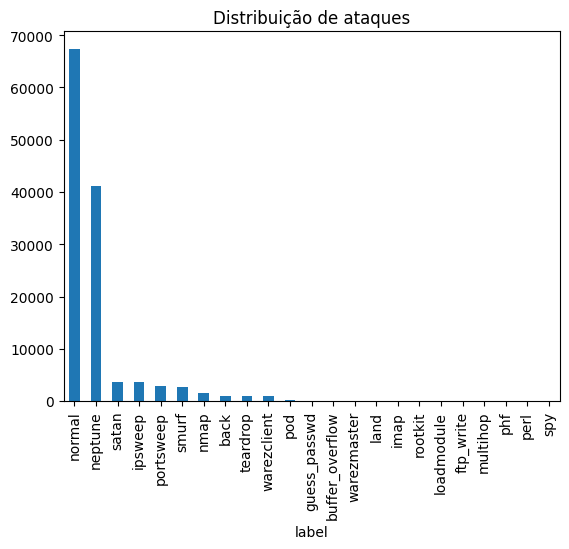
\includegraphics[width=\columnwidth]{distribuicao_ataques.png}
  \caption{Distribuição dos rótulos originais no \cod{KDDTrain+}.}
  \label{fig:distribuicao}
\end{figure}

% =============================================================================
\subsection{MVP1: Redução de Dimensionalidade}

Três técnicas complementares foram aplicadas. Primeiro, a matriz de correlação de
\en{Pearson} entre os atributos numéricos e o rótulo binário, para identificar
redundância e os atributos mais associados a ataques. Segundo, a Análise de
Componentes Principais (PCA), precedida de padronização por \en{StandardScaler}
(média zero e desvio padrão um), já que o PCA é sensível à escala; foi medido o
número de componentes necessários para reter 95\% da variância e gerada uma
projeção em duas dimensões para inspeção visual. Terceiro, a seleção por
importância: uma \en{Decision Tree} foi ajustada sobre os dados padronizados, os
atributos foram ordenados por importância (redução de impureza de Gini) e a mesma
árvore foi retreinada com os $k$ atributos mais importantes, para
$k = 5, \dots, 38$, registrando a acurácia de cada configuração.

% =============================================================================
\subsection{MVP1: Treinamento e Avaliação}

Cinco algoritmos foram comparados, todos com \cod{random\_state = 42}
(Tabela~\ref{tab:algoritmos}). O \cod{KDDTrain+} foi dividido em 80\% para treino
e 20\% para validação, de forma estratificada pelo rótulo. Foram medidas
acurácia, precisão, \en{recall}, \en{F1-score} e os tempos de treino e de predição,
estes últimos relevantes porque o objetivo final é a operação em tempo real.

O melhor modelo da validação foi então retreinado sobre todo o \cod{KDDTrain+} e
avaliado no \cod{KDDTest+}. Essa segunda avaliação é a mais importante do MVP1: o
\cod{KDDTest+} contém tipos de ataque que não existem no treino, o que aproxima o
teste da situação real de um IDS diante de ataques novos.

\begin{table}[H]
\centering
\footnotesize
\renewcommand{\arraystretch}{1.05}
\setlength{\tabcolsep}{2pt}
\begin{tabularx}{\linewidth}{
>{\hsize=0.7\hsize}X
>{\hsize=1.15\hsize}X
>{\hsize=1.15\hsize}X}
\toprule
\textbf{Algoritmo} & \textbf{Definição} \cite{IBM2026Supervised} & \textbf{Motivação} \\
\midrule
\en{Decision Tree} & Regras lógicas em fluxograma que dividem os dados. & Interpretável, baixo custo de predição. \\
\addlinespace
\en{Random Forest} & Combina várias árvores por votação. & Robusto e preciso, porém mais custoso. \\
\addlinespace
KNN ($k=5$) & Classifica pelos vizinhos mais próximos. & \en{Baseline} não paramétrico. \\
\addlinespace
\en{Logistic Regression} & Estima a probabilidade da classe. & \en{Baseline} linear, rápido. \\
\addlinespace
SVM (linear) & Hiperplano de máxima margem. & Eficaz em alta dimensão, lento em lote. \\
\bottomrule
\end{tabularx}
\caption{Algoritmos supervisionados avaliados no MVP1.}
\label{tab:algoritmos}
\end{table}

% =============================================================================
\subsection{MVP2: Arquitetura Geral}

O MVP2 é um NIDS que observa uma cópia passiva do tráfego e classifica cada fluxo
em uma cascata de dois modelos (Figura~\ref{fig:arquitetura}). O Estágio 1 é não
supervisionado porque não existe rótulo no tráfego de produção; ele funciona como
peneira, com \en{recall} alto e precisão baixa. O Estágio 2 é supervisionado e
opera apenas sobre os alertas do Estágio 1, com dois objetivos: recuperar formas
de ataque conhecidas que o Estágio 1 não enxerga e separar ataque real de anomalia
benigna. Os rótulos do Estágio 2 vêm do \en{golden set} e dos vereditos do analista.

\begin{figure*}[t]
  \centering
  \resizebox{\textwidth}{!}{% Arquitetura do MVP2 (largura total da página).
% Três faixas: detecção (cima), ciclo de vida do Estágio 1 (meio),
% refinamento supervisionado (baixo).
\begin{tikzpicture}[
  every node/.style={font=\scriptsize},
  proc/.style={rectangle, draw, rounded corners=2pt, fill=azulFEI!8,
               text width=2.5cm, align=center, minimum height=1.0cm, inner sep=2pt},
  dado/.style={cylinder, shape border rotate=90, aspect=0.18, draw, fill=gray!10,
               text width=2.4cm, align=center, minimum height=1.0cm, inner sep=1pt},
  ator/.style={rectangle, draw, thick, text width=2.3cm, align=center,
               minimum height=0.9cm, inner sep=2pt},
  zona/.style={draw=gray, dashed, rounded corners=4pt, inner sep=7pt},
  rot/.style={font=\scriptsize\sffamily\bfseries, text=gray},
  arrow/.style={-{Stealth[length=4pt]}},
  lbl/.style={font=\tiny, fill=white, inner sep=1pt}
]
  % ---------------- faixa 1: detecção em tempo real (y = 0)
  \node (span)   [ator] at (0,0)    {Porta espelho (SPAN) ou \en{bridge}};
  \node (det)    [proc] at (3.4,0)  {\cod{netanomaly\_live}\\extração de fluxos\\(janela de 10 s)};
  \node (e1)     [proc] at (6.8,0)  {\textbf{Estágio 1}\\\en{Isolation Forest}\\+ árvore \en{surrogate}};
  \node (sink)   [proc] at (10.2,0) {\cod{sink.py}\\percentil contra a grade do treino};
  \node (alerts) [dado] at (13.6,0) {\cod{na.alerts}\\(\en{hypertable})};

  % ---------------- faixa 2: ciclo de vida do Estágio 1 (y = -2.9)
  \node (pool)   [dado] at (10.2,-2.9) {\en{Pool} de \en{parquets} + \cod{feature\_windows}};
  \node (cand)   [proc] at (6.8,-2.9)  {\cod{lifecycle}\\\cod{candidate}\\(diário, automático)};
  \node (gate)   [proc] at (3.4,-2.9)  {Portão por cenário\\(\cod{v\_gate\_verdict})};
  \node (prom)   [ator] at (0,-2.9)    {Promoção manual\\(troca atômica)};
  \node (gold)   [dado] at (3.4,-4.5)  {\en{Golden set}\\(cenários rotulados)};

  % ---------------- faixa 3: refinamento supervisionado (y = -6.6)
  \node (e2)     [proc] at (13.6,-6.6) {\textbf{Estágio 2}\\SVM linear\\(\cod{netclassify})};
  \node (fila)   [dado] at (10.2,-6.6) {Predições e fila por margem};
  \node (ana)    [ator] at (6.8,-6.6)  {Analista\\(painel Grafana)};
  \node (ver)    [dado] at (3.4,-6.6)  {\cod{na.verdicts}};
  \node (final)  [dado] at (0,-6.6)    {Classificação final consolidada};

  % setas: detecção
  \draw[arrow] (span) -- (det);
  \draw[arrow] (det) -- (e1);
  \draw[arrow] (e1) -- node[lbl, above=2pt]{escore} (sink);
  \draw[arrow] (sink) -- node[lbl, above=2pt]{$p \geq 0{,}95$} (alerts);

  % setas: ciclo de vida
  \draw[arrow] (sink) -- node[lbl, right=2pt, align=left]{janelas de\\13 min} (pool);
  \draw[arrow] (pool) -- node[lbl, below=3pt, align=center]{quarentena 7 d\\meia-vida 14 d} (cand);
  \draw[arrow] (cand) -- (gate);
  \draw[arrow] (gold) -- (gate);
  \draw[arrow] (gate) -- node[lbl, above=2pt]{aprovado} (prom);
  \draw[arrow] (prom.north) -- ++(0,0.75) -| node[lbl, pos=0.3, above]{novo \texttt{current\_flow.joblib}} (e1.south);

  % setas: refinamento
  \draw[arrow] (alerts) -- node[lbl, right=2pt]{alertas} (e2);
  \draw[arrow] (e2) -- (fila);
  \draw[arrow] (fila) -- node[lbl, above=2pt]{menor margem} (ana);
  \draw[arrow] (ana) -- node[lbl, above=2pt]{veredito} (ver);
  \draw[arrow] (ver.south) -- ++(0,-0.55) -| node[lbl, pos=0.25, below]{rótulos para retreino} (e2.south);
  \draw[arrow] (ver) -- (final);
  \draw[arrow] (fila.north) -- ++(0,0.55) -| node[lbl, pos=0.25, above]{predição (sem veredito)} (final.north);

  \begin{scope}[on background layer]
    \node[zona, fit=(span)(alerts)] (z1) {};
    \node[zona, fit=(prom)(pool)(gold)] (z2) {};
    \node[zona, fit=(final)(e2)] (z3) {};
  \end{scope}
  \node[rot, anchor=south east] at (z1.north east) {detecção em tempo real};
  \node[rot, anchor=south east] at (z2.south east) {ciclo de vida do Estágio 1};
  \node[rot, anchor=north west] at (z3.south west) {refinamento supervisionado};
\end{tikzpicture}
}
  \caption{Arquitetura do MVP2: detecção em tempo real, refinamento supervisionado e ciclo de vida do modelo do Estágio 1.}
  \label{fig:arquitetura}
\end{figure*}

Os componentes de \en{software} são:
\begin{itemize}
  \item \cod{netanomaly.py}: extração de atributos, treino do Estágio 1, métricas e
  rotulagem do CIC-IDS-2017 pelo cronograma oficial;
  \item \cod{netanomaly\_live.py}: analisador em tempo real, que aplica o modelo
  congelado a janelas de 10 s;
  \item \cod{sink.py}: persistência, que grava janelas no \en{pool} de treino e
  alertas no banco;
  \item \cod{lifecycle.py}: ciclo de vida do Estágio 1 (\en{pool}, candidato,
  portão, promoção, despejo, adoção);
  \item \cod{netclassify.py}: Estágio 2 (veredito, treino, avaliação, promoção,
  predição e fila de revisão);
  \item \cod{migrations/}: esquema PostgreSQL/TimescaleDB, versionado por migração.
\end{itemize}

% =============================================================================
\subsection{MVP2: Extração de Atributos}

Os atributos do NSL-KDD não podem ser reproduzidos a partir de um \en{pcap}
arbitrário: vários dependem de inspeção de conteúdo e de contadores internos do
sensor original. Por isso o MVP2 define seu próprio vetor, calculável diretamente
dos cabeçalhos dos pacotes. O MVP1 contribuiu com a ordem de grandeza (17
atributos) e com a evidência de que volume, contagem e taxa de erro de conexão são
os sinais mais discriminantes. Duas visões são suportadas
(Tabela~\ref{tab:atributos}): por fluxo, agregando a 5-tupla bidirecional, e por
\en{host}, agregando por IP de origem para capturar o leque de conexões
(\en{fan-out}) típico de varreduras. A visão por fluxo foi a exercitada de ponta a
ponta.

\begin{table}[H]
\centering
\footnotesize
\setlength{\tabcolsep}{3pt}
\begin{tabularx}{\columnwidth}{l X}
\toprule
\textbf{Grupo} & \textbf{Atributos} \\
\midrule
\multicolumn{2}{l}{\textit{Visão por fluxo (17)}} \\
Volume      & \cod{n\_packets}, \cod{n\_bytes}, \cod{duration}, \cod{bytes\_per\_sec}, \cod{pkts\_per\_sec} \\
Tamanho     & \cod{mean\_len}, \cod{std\_len}, \cod{min\_len}, \cod{max\_len} \\
Tempo       & \cod{mean\_iat}, \cod{std\_iat} (intervalo entre pacotes) \\
Flags TCP   & \cod{syn\_ratio}, \cod{ack\_ratio}, \cod{fin\_ratio}, \cod{rst\_ratio}, \cod{psh\_ratio}, \cod{syn\_no\_ack} \\
\midrule
\multicolumn{2}{l}{\textit{Visão por host de origem (11)}} \\
Leque       & \cod{n\_dst}, \cod{n\_dports}, \cod{dports\_per\_dst}, \cod{pkts\_per\_dst} \\
Volume      & \cod{h\_packets}, \cod{h\_bytes}, \cod{h\_pkts\_per\_sec} \\
Handshake   & \cod{h\_syn\_ratio}, \cod{h\_ack\_ratio}, \cod{h\_rst\_ratio}, \cod{syn\_ack\_gap} \\
\bottomrule
\end{tabularx}
\caption{Vetores de atributos do MVP2.}
\label{tab:atributos}
\end{table}

% =============================================================================
\subsection{MVP2: Estágio 1 --- Detector e Explicação}

O detector é um \cod{StandardScaler} seguido de um \cod{IsolationForest} com 200
árvores, ambos ajustados com pesos por amostra iguais ao peso de recência da
janela de origem (Seção~III-H). O escore é invertido para que valores maiores
signifiquem mais anomalia, e o limiar $\tau$ é o quantil \emph{ponderado} do
escore de treino:

\begin{equation}
  s(x) = -\,\mathrm{score}(x), \qquad
  \tau = Q_w\!\left(1 - c\right),
  \label{eq:limiar}
\end{equation}

\noindent em que $c$ é o \en{contamination} e $Q_w$ é o quantil calculado sobre a
distribuição acumulada ponderada pelos pesos $w$. Usar o quantil simples com
pesos no ajuste faria o limiar responder a amostras que o modelo praticamente
ignorou. O limiar é \emph{congelado} no artefato: o analisador ao vivo nunca o
recalcula, pois isso faria a taxa de alerta depender da composição da janela
corrente e não do treino.

Junto ao limiar, o artefato guarda uma grade de 1.001 quantis do escore de treino.
O percentil de cada fluxo é calculado contra essa grade, e não contra os demais
fluxos da mesma janela. Percentil relativo à janela produziria alerta por
construção: em uma janela sem ataque algum, o “1\% mais anômalo” é tráfego
normal. Contra a grade do treino, uma janela tranquila não gera alerta, e o
percentil fica disponível imediatamente, sem esperar a janela fechar.

Para a explicabilidade, uma \cod{DecisionTreeClassifier} de profundidade 4 é
treinada sobre os atributos \emph{não escalados}, tendo como alvo o rótulo
atribuído pelo próprio \en{Isolation Forest}. A regra do caminho percorrido por
cada alerta (por exemplo, \cod{n\_dports > 50 e duration <= 2,1}) é exibida ao
analista em unidades reconhecíveis. A árvore explica, mas não decide.

% =============================================================================
\subsection{MVP2: Estágio 2 --- Refinador Supervisionado}

O Estágio 2 usa \cod{StandardScaler} e \cod{LinearSVC} com $C=1$ e
\cod{class\_weight="balanced"}, porque ataque é a classe minoritária. Os
atributos de entrada são os 17 do fluxo; o escore do Estágio 1 está
disponível em cada alerta para versões futuras. O SVM linear foi escolhido, em vez
de uma clusterização pura, porque sua \cod{decision\_function} fornece a
distância com sinal ao hiperplano, usada para priorizar a revisão. A clusterização
fica reservada como apoio à rotulagem em lote.

\textbf{Partida a frio.} Uma instalação nova não tem nenhum veredito. O primeiro
hiperplano é treinado sobre o \en{golden set} (capturas rotuladas como ataque ou
benigno) e entra em produção com a decisão registrada como \emph{adotado}, pois não
passou por portão. Os vereditos do analista são somados ao treino à medida que
chegam e valem como rótulo da rede real.

\textbf{Operação.} O comando \cod{predict} aplica o SVM promovido a cada alerta e
grava a classe predita, o valor de decisão e a margem. A fila de revisão é
ordenada por margem crescente: os casos mais próximos da fronteira aparecem
primeiro, que é onde o veredito mais move o hiperplano (aprendizado ativo por
incerteza \cite{Settles2009Active}). Para o painel, uma projeção PCA em duas
dimensões é ajustada no treino e congelada no artefato, de modo que pontos de
janelas diferentes sejam comparáveis.

\textbf{Anotar, não suprimir.} O Estágio 2 reordena e anota a fila, mas não
descarta alerta automaticamente. Supressão automática criaria falso negativo
silencioso justamente quando o modelo, recém-treinado com poucos vereditos, ainda
erra mais. A classificação final consolidada segue a precedência
\emph{veredito $>$ Estágio 2 $>$ apenas Estágio 1 (pendente)}.

\textbf{Vereditos.} Cada veredito guarda uma cópia do vetor de atributos, porque a
retenção de alertas é de 180 dias e o rótulo precisa sobreviver ao alerta que o
originou. Revisões não sobrescrevem: criam uma nova linha que aponta para a
anterior, preservando divergências entre analistas como informação.

% =============================================================================
\subsection{MVP2: Ciclo de Vida e Defesa contra Envenenamento}

A decisão central do ciclo de vida é que o detector \textbf{nunca é retreinado na
janela de tráfego mais recente}. O \en{Isolation Forest} aprende como normal a
massa dos dados que recebe; se a janela contém ataque, o ataque passa a ser normal
e deixa de ser marcado. Isso é explorável de forma gradual: um canal de comando e
controle (C2) com batida de 6~h é absorvido um pouco mais a cada retreino, sem que
o atacante precise evadir nada \cite{Biggio2012Poisoning}. O que o dado recente
compra de fato é redução de falso positivo (servidor novo, mudança de horário de
\en{backup}). Por isso o treino ocorre sobre um \en{pool} curado
(Figura~\ref{fig:ciclo}):

\begin{itemize}
  \item \textbf{Janela de \en{pool}:} o \cod{sink} agrupa os fluxos em janelas de
  780 s (13 min), alinhadas da mesma forma para captura ao vivo e para
  \en{pcap} histórico. É uma cadência distinta da janela de análise de 10 s, que
  só determina a latência do alerta.
  \item \textbf{Quarentena:} a janela só entra no \en{pool} depois de 7 dias sem
  indicador de comprometimento (IOC) retroativo.
  \item \textbf{Recência:} cada janela recebe peso
  $w = 0{,}5^{\,(t_{\max}-t)/h}$, com meia-vida $h = 14$ dias, normalizado pela
  janela mais nova do \en{pool} --- sem a normalização, uma captura histórica teria
  peso da ordem de $10^{-64}$. Janelas com $w < 0{,}05$ são descartadas. A
  amostragem (limitada a 2 milhões de linhas) é proporcional ao tamanho da janela e
  serve só para limitar memória; a recência entra apenas pelo \cod{sample\_weight},
  para não ser aplicada duas vezes.
  \item \textbf{Despejo e procedência:} cada modelo registra quais janelas o
  treinaram. Descoberto um comprometimento, as janelas do período são despejadas,
  a consulta \cod{v\_models\_contaminados} lista os modelos que as absorveram e um
  novo candidato é treinado sem elas --- algo impossível em aprendizado incremental.
  \item \textbf{Homogeneidade:} janelas com contratos de atributos diferentes não
  são misturadas, pois isso geraria um modelo cujo vetor de entrada não existe.
\end{itemize}

\begin{figure}[H]
  \centering
  % Estados de uma janela de tráfego e os três relógios do ciclo de vida
\resizebox{\columnwidth}{!}{%
\begin{tikzpicture}[
  node distance=0.45cm and 0.55cm,
  every node/.style={font=\scriptsize},
  est/.style={rectangle, draw, rounded corners=6pt, fill=azulFEI!8,
              text width=1.6cm, align=center, minimum height=0.8cm, inner sep=2pt},
  mau/.style={est, fill=red!10},
  arrow/.style={-{Stealth[length=4pt]}},
  lbl/.style={font=\tiny, align=center}
]
  \node (jan)  [est] {Janela capturada (13 min)};
  \node (qua)  [est, right=of jan] {Quarentena};
  \node (ati)  [est, right=of qua] {\en{Pool} ativo};
  \node (pes)  [est, right=of ati] {Peso $\to$ 0 (cauda)};
  \node (des)  [mau, below=0.9cm of ati] {Despejada};
  \node (mod)  [mau, right=of des] {Modelos contaminados};

  \draw[arrow] (jan) -- (qua);
  \draw[arrow] (qua) -- node[lbl, above]{7 dias sem\\IOC} (ati);
  \draw[arrow] (ati) -- node[lbl, above]{$w<0{,}05$} (pes);
  \draw[arrow] (qua.south) |- node[lbl, pos=0.3, left]{IOC\\retroativo} (des.west);
  \draw[arrow] (ati) -- node[lbl, right]{IOC} (des);
  \draw[arrow] (des) -- node[lbl, above]{procedência} (mod);
\end{tikzpicture}%
}

  \caption{Estados de uma janela de tráfego no \en{pool} de treino.}
  \label{fig:ciclo}
\end{figure}

O ciclo é regido por três relógios separados: a árvore \en{surrogate} é
atualizada a cada janela; um candidato é treinado e medido diariamente, de forma
automática; e a promoção para produção é semanal ou sob demanda e
\textbf{sempre manual}. Um portão que se auto-aprova não é portão: com poucos
cenários no \en{golden set}, ele daria aparência de verificação ao que não foi
verificado. Ao promover, o modelo anterior e as árvores que o descreviam são
aposentados e o artefato é trocado por \cod{rename()} atômico de um \en{symlink},
que o detector recarrega sem reinício. O analista também pode pedir retreino
manual, mas o pedido registra junto o número de quase-acertos que o justifica ---
alertas confirmados como ataque que ficaram abaixo do corte, medidos pela consulta
\cod{v\_stage1\_near\_misses}.

% =============================================================================
\subsection{MVP2: Golden Set e Portão de Promoção}

O \en{golden set} é um conjunto de capturas rotuladas, organizado por cenário
(Tabela~\ref{tab:cenarios}). As capturas podem ser registradas manualmente, a
partir de testes de intrusão feitos pelo próprio operador, ou derivadas do
cronograma oficial de ataques do CIC-IDS-2017 \cite{Sharafaldin2018Toward}.
Todo candidato é avaliado por captura, por cenário e no agregado.

\begin{table}[H]
\centering
\footnotesize
\setlength{\tabcolsep}{3pt}
\begin{tabularx}{\columnwidth}{l X c c}
\toprule
\textbf{Cenário} & \textbf{Descrição} & \textbf{E1} & \textbf{E2} \\
\midrule
recon        & Varredura de portas e \en{hosts} (nmap) & 0,90$^*$ & 0,90 \\
brute\_force & Força bruta em SSH, FTP, HTTP & --- & 0,85 \\
exfil        & Exfiltração por canal incomum & --- & 0,80 \\
beacon\_1h   & C2 com batida horária & --- & 0,75 \\
beacon\_6h   & C2 com batida de 6~h & --- & 0,60 \\
lateral      & Movimento lateral (SMB, RDP) & --- & 0,80 \\
benigno      & Controle limpo: mede falso positivo & FPR & FPR \\
\bottomrule
\end{tabularx}
\caption{Cenários do \en{golden set} e piso de \en{recall} exigido por estágio. $^*$não obrigatório até haver captura real.}
\label{tab:cenarios}
\end{table}

Um candidato é reprovado se \emph{qualquer} cenário isolado: (i) cair mais de
0,10 de \en{recall} em relação ao modelo em produção; (ii) ficar abaixo do piso
absoluto do cenário; ou (iii) exceder 2\% de falso positivo no controle benigno. O
terceiro critério impede que um candidato degenerado, que alerta em tudo, passe
com \en{recall} 1,00 em todos os cenários. A avaliação é por cenário, e não
agregada, porque o envenenamento lento aparece como a queda de \emph{um} cenário
específico, que a média esconde.

Os pisos são definidos por estágio. O \en{Isolation Forest} é estruturalmente
cego a ataques volumosos e homogêneos (Seção~IV-D); exigir \cod{brute\_force} dele
tornaria o portão do Estágio 1 impossível de passar. Assim, o Estágio 1 é cobrado
de varredura e falso positivo, e os ataques densos são cobrados do Estágio 2.

\textbf{Adoção.} Uma instalação nova enfrenta um impasse circular: o detector
precisa de modelo promovido, a promoção precisa de candidato, o candidato precisa
de \en{pool}, e o \en{pool} é alimentado pelo detector. O comando \cod{adopt} rompe o
círculo com um modelo treinado fora do ciclo: valida o contrato de atributos, gera
a grade de percentis a partir da captura de treino, semeia o \en{pool} com essa
captura (registrando a procedência) e registra o modelo como \emph{adotado}. O
detector, por sua vez, não treina sozinho: em uma instância vazia ele aguarda,
explicando o que falta, pois treinar no tráfego que estiver passando é exatamente
o caminho do envenenamento.

% =============================================================================
\subsection{MVP2: Persistência}

O banco é PostgreSQL 17 com a extensão TimescaleDB, organizado no esquema
\cod{na} (14 tabelas e 11 consultas, \en{views}, após as migrações). Quatro
decisões estruturam o esquema:

\begin{enumerate}
  \item \textbf{Fluxos não vão para o banco.} Uma captura de 10~GB gera milhões de
  fluxos; o treino quer formato colunar comprimido. Os fluxos ficam em arquivos
  \en{Parquet} em disco, e o banco guarda um índice deles (\cod{feature\_windows}),
  com estado de quarentena e despejo. Só o que vira alerta entra como linha.
  \item \textbf{O corte do analista é aplicado na consulta.} Há dois limiares: o
  piso de gravação (percentil 0,95, fixo) e o corte de exibição (0,99, ajustável).
  Como o corte é aplicado em uma \en{view}, alterá-lo tem efeito retroativo sem
  reprocessar nada.
  \item \textbf{Escore e percentil são guardados juntos.} O percentil permite ao
  analista raciocinar em porcentagem; o escore contínuo alimenta o Estágio 2.
  \item \textbf{Sem chave estrangeira para alertas.} A tabela de alertas é uma
  \en{hypertable} com retenção de 180 dias; vereditos e predições referenciam o
  alerta com integridade garantida pela aplicação.
\end{enumerate}

Os parâmetros operacionais (limiares, quarentena, meia-vida, tolerâncias do
portão) ficam em uma tabela editável com histórico de alterações por gatilho. As
migrações são aplicadas uma única vez cada por um controlador próprio, cada uma em
transação junto com seu registro; se uma falha, o contêiner aborta de propósito.

% =============================================================================
\subsection{MVP2: Implantação em Contêineres}

Uma única imagem (\cod{python:3.13-slim}) serve aos papéis de detector, treinador
e utilitários, garantindo a mesma versão de \en{scikit-learn} em todos --- requisito,
pois o artefato \cod{.joblib} é serializado por versão. Nenhum contêiner roda como
\en{root}: as capacidades \cod{cap\_net\_raw} e \cod{cap\_net\_admin} são
atribuídas ao binário \cod{tcpdump} como \en{file capabilities}, de modo que um
processo de UID 1000 abre o \en{socket} de captura. A Tabela~\ref{tab:servicos}
resume os serviços do \en{Docker Compose}.

\begin{table}[H]
\centering
\footnotesize
\setlength{\tabcolsep}{3pt}
\begin{tabularx}{\columnwidth}{l l X}
\toprule
\textbf{Serviço} & \textbf{Perfil} & \textbf{Função} \\
\midrule
banco            & ---              & TimescaleDB, porta só em \cod{127.0.0.1} \\
treinador        & ---              & Migrações e relógio diário de candidatos \\
detector         & sensor           & Captura em \cod{network\_mode: host} \\
detector-isolado & sensor-isolado   & NIC dedicada via \en{macvlan passthru} \\
replay           & replay           & Reprocessa um \en{pcap}, sem captura \\
grafana          & painel           & Painéis dos Estágios 1, 2 e resultado final \\
\bottomrule
\end{tabularx}
\caption{Serviços do \en{Docker Compose} e perfis de ativação.}
\label{tab:servicos}
\end{table}

Um contêiner só enxerga o tráfego que chega ao seu \en{namespace} de rede. Por
isso o \en{macvlan} em modo \en{bridge}, opção mais intuitiva, não serve para IDS:
o \en{kernel} entrega ao contêiner apenas o tráfego destinado ao seu próprio
endereço MAC. As opções válidas são o modo \en{host}, que vê uma interface
promíscua ligada à porta espelho (SPAN) do \en{switch}, e o \en{macvlan
passthru}, que entrega a placa inteira ao contêiner. O arranjo recomendado usa
duas interfaces: uma de gerência, com IP, e uma de captura, sem IP e em modo
promíscuo. No laboratório, a máquina virtual do sensor roda sobre Proxmox, com a
interface em modo promíscuo e a \en{bridge} virtual com \en{ageing time} zero, o
que faz a \en{bridge} repassar todos os quadros a todas as portas, à maneira de
um \en{hub}.

Os painéis do Grafana leem diretamente o banco e cobrem: o Estágio 1 (alertas
acima do corte, quase-acertos, janelas no \en{pool}, portão do último candidato);
o Estágio 2 (dispersão do SVM em PCA 2D, desempenho por cenário, fila por margem);
e o resultado final consolidado, com a classificação ao longo do tempo e o acerto
contra o rótulo real quando disponível. A arquitetura prevista para o
\en{front-end} é híbrida: parâmetros editados por um painel de formulários do
próprio Grafana, e a tela de veredito como aplicação própria na mesma origem,
via \en{proxy} reverso, evitando desligar a sanitização de HTML do Grafana.

% =============================================================================
\subsection{MVP2: Protocolo de Avaliação}

Duas fontes de dados foram usadas, com papéis distintos:

\begin{itemize}
  \item \textbf{CIC-IDS-2017} \cite{Sharafaldin2018Toward}: capturas reais
  (\en{pcap}) rotuladas pelo cronograma oficial dos ataques, com tratamento de
  NAT. O ataque FTP-Patator, da terça-feira, foi usado como \en{golden set} real de
  \cod{brute\_force}.
  \item \textbf{Gerador sintético} (\cod{scripts/gerar\_sintetico.py}): produz
  \en{pools} e capturas de varredura, beacon e tráfego normal com distribuições
  controladas. Os números obtidos com ele medem o \emph{mecanismo} (portão,
  quarentena, despejo), nunca a capacidade real de detecção.
\end{itemize}

As métricas principais são o \en{recall} por cenário e a taxa de falso positivo
(FPR) no controle benigno; ROC-AUC e precisão média (AP) complementam a análise do
Estágio 1. Os experimentos de envenenamento usam 5 sementes aleatórias, com o
gerador re-semeado antes de cada \en{pool}, porque seu estado compartilhado faria a
composição do \en{pool} depender da ordem das chamadas. Por fim, uma demonstração de
ponta a ponta (\cod{scripts/demo\_ataque.sh}) sobe um atacante e uma vítima em
contêineres, executa uma varredura \cod{nmap} e verifica se o pipeline grava
alertas usando o mesmo modelo, banco e código da produção.

\section{Resultados e Discussão}

% =============================================================================
\subsection{MVP1: Análise Exploratória}

A matriz de correlação (Figura~\ref{fig:matriz_corr}) mostra blocos de atributos
fortemente correlacionados entre si, em especial as taxas de erro de conexão e as
contagens por \en{host} de destino. Os atributos mais correlacionados com o rótulo
de ataque são as taxas de erro SYN --- \cod{dst\_host\_srv\_serror\_rate} (0,655),
\cod{dst\_host\_serror\_rate} (0,652), \cod{serror\_rate} (0,651) e
\cod{srv\_serror\_rate} (0,648) --- seguidas de \cod{count} (0,576). São
exatamente os sinais de inundação SYN, como o \en{neptune}, que responde por 70\% dos
ataques do treino.

\begin{figure}[H]
  \centering
  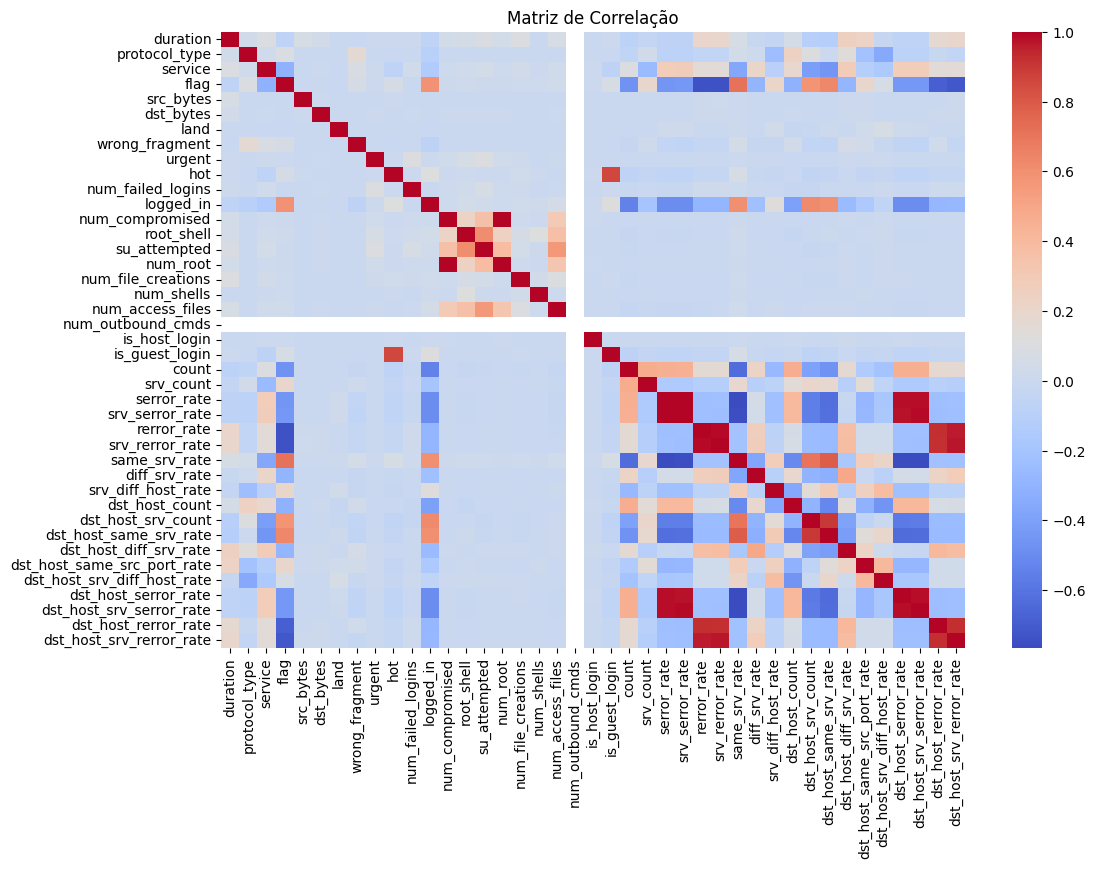
\includegraphics[width=0.95\columnwidth]{matriz_corr.png}
  \caption{Matriz de correlação de \en{Pearson} dos atributos numéricos do NSL-KDD.}
  \label{fig:matriz_corr}
\end{figure}

O PCA precisou de 22 dos 36 componentes para reter 95,43\% da variância
(Figura~\ref{fig:pca_variancia}). A projeção nos dois primeiros componentes
(Figura~\ref{fig:pca_classes}) mostra que DoS e \en{Probe} ocupam regiões
distintas do tráfego normal, enquanto R2L e U2R se sobrepõem a ele --- coerente
com a natureza desses ataques, que se parecem com sessões legítimas no nível de
conexão.

\begin{figure}[H]
  \centering
  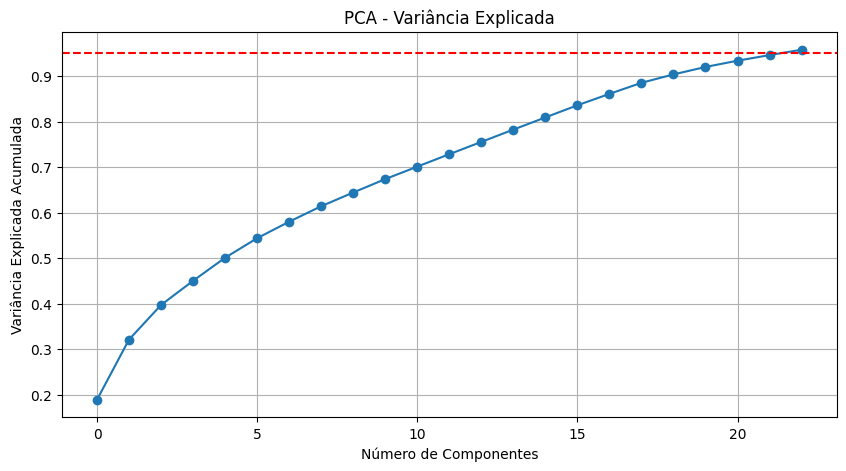
\includegraphics[width=\columnwidth,height=5cm]{pcaXvariancia.png}
  \caption{Variância explicada acumulada em função do número de componentes do PCA.}
  \label{fig:pca_variancia}
\end{figure}

\begin{figure}[H]
  \centering
  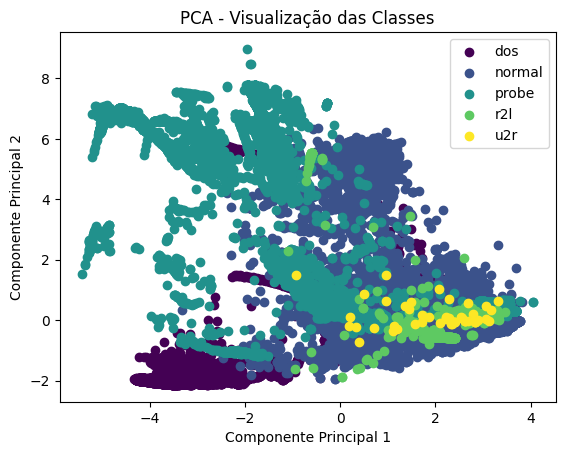
\includegraphics[width=0.95\columnwidth]{pca_classes.png}
  \caption{Projeção nos dois primeiros componentes principais, por categoria.}
  \label{fig:pca_classes}
\end{figure}

% =============================================================================
\subsection{MVP1: Comparação de Algoritmos}

A Tabela~\ref{tab:mvp1} resume a comparação na partição de validação. Os modelos
baseados em árvore dominam as métricas de classificação, mas o custo
computacional separa os candidatos. O \en{Random Forest} tem o maior
\en{F1-score} (0,9984), porém treina em 6,7~s e prediz em 0,20~s. A
\en{Decision Tree} fica a 0,0007 de distância no \en{F1-score}, treina 9 vezes mais
rápido e prediz 56 vezes mais rápido (3,5~ms para cerca de 25 mil registros). O KNN
não tem custo de treino, mas leva 16~s para predizer, inviável em fluxo contínuo,
e o SVM com \en{kernel} linear em lote foi o mais lento em ambas as fases (198~s de
treino). Pelo equilíbrio entre acurácia e latência, a \en{Decision Tree} foi
selecionada no MVP1.

\begin{table}[H]
\centering
\footnotesize
\setlength{\tabcolsep}{2.5pt}
\begin{tabular}{l c c c c r r}
\toprule
\textbf{Modelo} & \textbf{Acc} & \textbf{Prec} & \textbf{Rec} & \textbf{F1} & \textbf{Treino (s)} & \textbf{Teste (s)} \\
\midrule
RF  & 0,9985 & 0,9991 & 0,9977 & 0,9984 &   6,70 &  0,196 \\
DT  & 0,9978 & 0,9977 & 0,9976 & 0,9977 &   0,72 &  0,004 \\
KNN & 0,9919 & 0,9900 & 0,9926 & 0,9913 &   0,00 & 16,014 \\
LR  & 0,9488 & 0,9576 & 0,9312 & 0,9442 &   1,89 &  0,002 \\
SVM & 0,9532 & 0,9658 & 0,9325 & 0,9489 & 198,34 &  7,605 \\
\bottomrule
\end{tabular}
\caption{Desempenho na validação (20\% estratificado do \cod{KDDTrain+}, 36 atributos padronizados).}
\label{tab:mvp1}
\end{table}

A seleção por importância mostrou que o sinal está concentrado em poucos
atributos: \cod{src\_bytes} sozinho responde por 74,9\% da importância da árvore,
os dois primeiros por 80\% e os cinco primeiros por 90\%
(Figura~\ref{fig:importancia}). Variando o número de atributos de 5 a 38
(Figura~\ref{fig:n_features}), a acurácia já é 0,9961 com 5 atributos e atinge o
máximo de 0,9980 com 17, com variação inferior a 0,0005 a partir daí. Os
17 atributos selecionados são, em ordem: \cod{src\_bytes},
\cod{dst\_host\_srv\_count}, \cod{count}, \cod{dst\_bytes},
\cod{dst\_host\_same\_src\_port\_rate}, \cod{num\_compromised},
\cod{dst\_host\_same\_srv\_rate}, \cod{srv\_count}, \cod{diff\_srv\_rate},
\cod{duration}, \cod{dst\_host\_count}, \cod{dst\_host\_rerror\_rate},
\cod{wrong\_fragment}, \cod{dst\_host\_diff\_srv\_rate},
\cod{dst\_host\_srv\_serror\_rate}, \cod{is\_guest\_login} e
\cod{dst\_host\_serror\_rate}. O resultado está em linha com a literatura, que
relata conjuntos de 9 a 20 atributos sem perda de desempenho
\cite{Thakkar2021Survey, Othman2018Intrusion, Rathore2016RealTime}.

\begin{figure}[H]
  \centering
  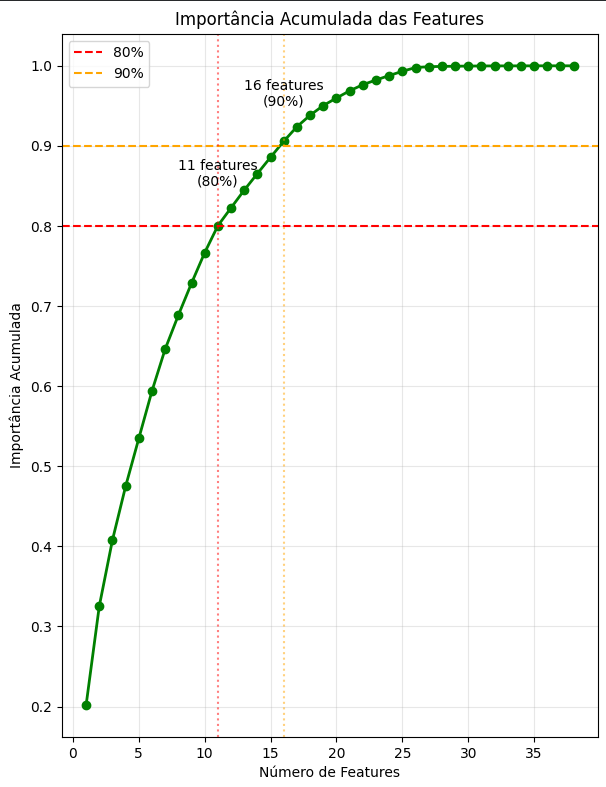
\includegraphics[width=\columnwidth,height=7.5cm]{Importancia_features.png}
  \caption{Importância dos atributos segundo a \en{Decision Tree}.}
  \label{fig:importancia}
\end{figure}

\begin{figure}[H]
  \centering
  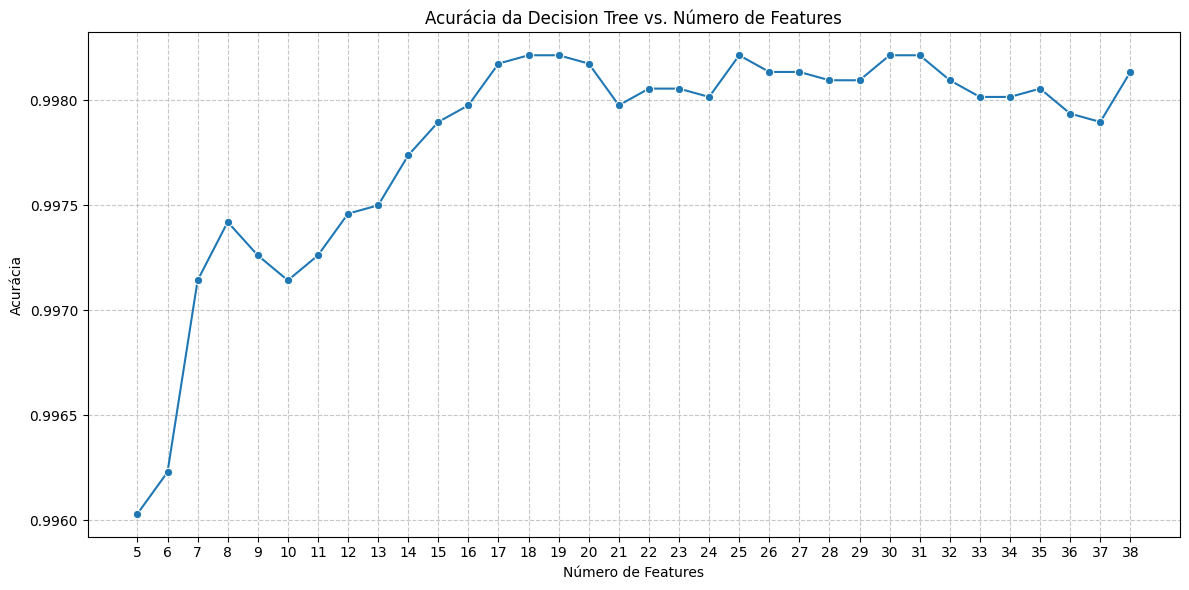
\includegraphics[width=\columnwidth,height=5cm]{decisiontree_features.png}
  \caption{Acurácia da \en{Decision Tree} em função do número de atributos mais importantes.}
  \label{fig:n_features}
\end{figure}

% =============================================================================
\subsection{MVP1: Generalização para Ataques Novos}

Retreinado sobre todo o \cod{KDDTrain+} e aplicado ao \cod{KDDTest+}, o melhor
modelo da validação (\en{Random Forest}) caiu para \textbf{77,92\% de acurácia} e
\textbf{63,22\% de \en{recall}}, mantendo precisão de 96,93\% (F1 = 0,7653). A
matriz de confusão (Figura~\ref{fig:confusao}) mostra que o erro é quase todo
falso negativo: 4.720 dos 12.833 ataques do teste foram classificados como
normais, contra apenas 257 falsos positivos.

\begin{figure}[H]
  \centering
  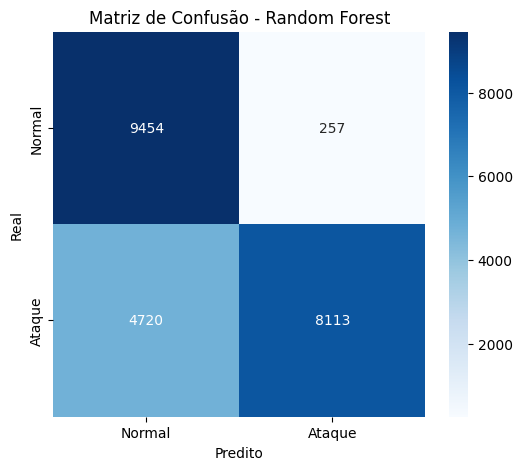
\includegraphics[width=0.75\columnwidth]{matriz_confusao_kddtest.png}
  \caption{Matriz de confusão do \en{Random Forest} no \cod{KDDTest+}.}
  \label{fig:confusao}
\end{figure}

Esse é o resultado mais importante do MVP1. A acurácia de 99,8\% mede a capacidade
de reconhecer ataques \emph{já vistos}; diante de tipos ausentes do treino, o
classificador supervisionado os trata como normais e falha em silêncio. O modelo
não “erra para o lado seguro”: quando não reconhece, declara benigno. A divisão
aleatória do próprio \cod{KDDTrain+}, prática comum na literatura, superestima
o desempenho real \cite{Sommer2010Outside}. Daí derivam três requisitos do MVP2:
(i) um detector não supervisionado, que não dependa de ter visto o ataque; (ii)
um classificador supervisionado alimentado continuamente por rótulos da própria
rede; e (iii) avaliação por cenário de ataque, e não por acurácia agregada.

% =============================================================================
\subsection{MVP2: Ponto Cego do Isolation Forest}

O Estágio 1 foi avaliado com o \en{golden set} real de FTP-Patator do CIC-IDS-2017:
3.958 fluxos de ataque contra 93.883 fluxos de fundo da mesma rede e horário,
com modelo treinado sobre 26.507 fluxos benignos da mesma captura. O resultado foi
\textbf{\en{recall} 0,00} contra o piso de 0,85 do cenário. O ROC-AUC de 0,781 e a
precisão média de 0,0887 (contra 0,0405 de base) indicam alguma separação, mas
para \emph{qualquer} nível de \en{recall} o custo é de 22\% de falso positivo: o
limiar que captura 50\% do ataque (0,4689) é praticamente o mesmo que captura 99\%
(0,4679), porque todos os fluxos de ataque recebem quase o mesmo escore.

O problema não está nos atributos. Contra a mediana benigna, o ataque tem duração
147 vezes maior, \cod{std\_iat} 68 vezes, \cod{mean\_iat} 13 vezes e
\cod{n\_packets} 7 vezes. A causa é estrutural: 3.958 fluxos quase idênticos formam
um aglomerado denso, e o \en{Isolation Forest} isola pontos \emph{raros}
(Equação~\ref{eq:if}). Quanto mais o atacante repete, mais normal ele fica. A
ordenação resultante é \emph{benigno atípico $>$ ataque $>$ benigno típico}, e
nenhum limiar separa as classes --- ajustar o \en{contamination} não resolve. É a
mesma família do beacon de 6~h: ataques cuja assinatura está na repetição ao longo
do tempo, e não no fluxo individual.

% =============================================================================
\subsection{MVP2: Estágio 2 Recupera os Ataques Densos}

Para validar a premissa do Estágio 2, um SVM linear foi treinado nos mesmos 17
atributos e avaliado em conjuntos de teste separados, cenário a cenário
(Tabela~\ref{tab:e2}). O classificador supervisionado recupera integralmente os
ataques densos que o \en{Isolation Forest} não vê, inclusive a força bruta.

\begin{table}[H]
\centering
\footnotesize
\begin{tabular}{l c c}
\toprule
\textbf{Cenário} & \textbf{\en{Isolation Forest}} & \textbf{SVM linear} \\
\midrule
recon            & 0,36  & 1,00  \\
beacon\_6h       & 0,08  & 1,00  \\
brute\_force     & 0,00  & 1,00  \\
\midrule
FPR (benigno)    & 0,001 & 0,000 \\
\bottomrule
\end{tabular}
\caption{\en{Recall} por cenário e taxa de falso positivo, mesmos atributos e dados.}
\label{tab:e2}
\end{table}

Esses valores devem ser lidos com cautela. São resultados \emph{em distribuição}:
o SVM foi testado sobre formas de ataque que viu rotuladas no treino. Como mostrou
o MVP1, um classificador supervisionado não generaliza para ataques novos --- que
continuam sendo responsabilidade do Estágio 1. Em produção, o rótulo vem do
analista, é ruidoso e é enviesado pelo que o Estágio 1 decidiu mostrar. A Tabela
não mede detecção geral; mede que os dois estágios são \emph{complementares}: o não
supervisionado pega o raro e o novo, o supervisionado pega o conhecido e o denso.

% =============================================================================
\subsection{MVP2: Contamination e Teto de Falso Positivo}

Em um \en{pool} majoritariamente limpo, a taxa de falso positivo do
\en{Isolation Forest} tende ao valor de \en{contamination}, que é literalmente a
fração que o modelo foi instruído a marcar. Medido no \en{golden set}: 0,03 $\to$
FPR 0,026; 0,01 $\to$ 0,006; 0,005 $\to$ 0,001. Consequentemente, se o teto de
falso positivo do portão for menor que o \en{contamination}, \emph{nenhum}
candidato passa, e o sintoma se parece com degradação do modelo quando é apenas
aritmética da configuração. A configuração inicial tinha exatamente esse defeito
(teto de 0,02 contra \en{contamination} de 0,03), e o comando de treino passou a
emitir um aviso nesse caso.

A faixa utilizável é estreita: com 0,03 o candidato reprova por falso positivo;
com 0,01 passa; com 0,005 reprova porque o \en{recall} de \cod{beacon\_1h} cai
para 0,04 e o de \cod{beacon\_6h} para 0,06, enquanto \cod{recon} permanece em
1,00. Beacon é anomalia sutil e precisa de limiar mais frouxo; varredura sobrevive
a qualquer limiar. Uma métrica agregada teria escondido essa diferença.

% =============================================================================
\subsection{MVP2: Explicação Não Mede Detecção}

Uma hipótese natural seria usar a fidelidade da árvore \en{surrogate} como
gatilho de retreino. A Tabela~\ref{tab:surrogate} mostra por que isso não
funciona: com o \en{pool} envenenado por 10\% de tráfego C2, a detecção dos beacons
foi a zero enquanto a fidelidade variou um décimo de ponto percentual.

\begin{table}[H]
\centering
\footnotesize
\setlength{\tabcolsep}{3pt}
\begin{tabular}{l c c c c}
\toprule
\textbf{Regime do \en{pool}} & \textbf{Fidelid.} & \textbf{F1} & \textbf{bcn1h} & \textbf{bcn6h} \\
\midrule
Limpo                   & 0,997 & 0,838 & 0,85 & 0,98 \\
Envenenado (10\% C2)    & 0,996 & 0,780 & \textbf{0,00} & \textbf{0,01} \\
Deriva legítima         & 0,997 & 0,827 & 0,70 & 0,92 \\
\bottomrule
\end{tabular}
\caption{Fidelidade da árvore \en{surrogate} contra \en{recall} real por cenário.}
\label{tab:surrogate}
\end{table}

Quando o C2 vira normal, a floresta deixa de marcá-lo e a árvore reproduz esse
silêncio com fidelidade perfeita: as duas concordam em estar erradas. Além disso,
a queda de F1 causada pelo envenenamento (0,058) é menor que o desvio entre
partições do modelo limpo (0,131), de modo que nenhum limiar separa os casos.
A validação do retreino precisa medir detecção por cenário --- que é o que o
portão faz.

% =============================================================================
\subsection{MVP2: Orçamento do Atacante contra o Portão}

Para medir a sensibilidade do portão, tráfego de beacon com período de 6~h foi
injetado em doses crescentes em um \en{pool} sintético de 120.000 fluxos, com 5
sementes, e cada candidato foi avaliado contra o mesmo \en{golden set}
(Tabela~\ref{tab:dose} e Figura~\ref{fig:dose}).

\begin{table}[H]
\centering
\footnotesize
\setlength{\tabcolsep}{3pt}
\begin{tabular}{r r c c r l}
\toprule
\textbf{Dose} & \textbf{$n$} & \textbf{bcn1h} & \textbf{bcn6h} & \textbf{$\Delta$1h} & \textbf{Portão} \\
\midrule
0,00\% &    0 & 0,891 & 0,984 & $+$0,000 & passa \\
0,05\% &   60 & 0,827 & 0,987 & $-$0,064 & passa \\
0,10\% &  120 & 0,645 & 0,976 & $-$0,246 & \textbf{reprova} \\
0,30\% &  360 & 0,159 & 0,948 & $-$0,732 & \textbf{reprova} \\
1,00\% & 1200 & 0,000 & 0,520 & $-$0,891 & \textbf{reprova} \\
\bottomrule
\end{tabular}
\caption{Curva dose-resposta do envenenamento (média de 5 sementes; desvio da base em bcn1h: $\pm$0,029).}
\label{tab:dose}
\end{table}

\begin{figure}[H]
\centering
\begin{tikzpicture}
\begin{axis}[
  width=\columnwidth, height=5.2cm,
  xmode=log, log basis x=10,
  xmin=0.03, xmax=1.3,
  ymin=0, ymax=1.05,
  xlabel={\scriptsize Dose de C2 no \en{pool} (\%)},
  ylabel={\scriptsize \en{Recall}},
  xtick={0.05,0.1,0.3,1}, xticklabels={{0,05},{0,10},{0,30},{1,00}},
  ticklabel style={font=\scriptsize},
  legend style={font=\scriptsize, at={(0.03,0.05)}, anchor=south west, draw=gray!50, fill=white},
  grid=major, grid style={gray!20},
]
  \fill[red!8] (axis cs:0.075,0) rectangle (axis cs:1.3,1.05);
  \node[font=\tiny, text=red!60!black, anchor=north east] at (axis cs:1.25,1.03) {portão reprova};
  \addplot[azulFEI, thick, mark=*, mark size=1.5pt] coordinates {(0.05,0.827) (0.1,0.645) (0.3,0.159) (1,0.000)};
  \addplot[gray, thick, dashed, mark=square*, mark size=1.5pt] coordinates {(0.05,0.987) (0.1,0.976) (0.3,0.948) (1,0.520)};
  \addplot[black, densely dotted] coordinates {(0.03,0.75) (1.3,0.75)};
  \legend{beacon\_1h, beacon\_6h, piso bcn1h}
\end{axis}
\end{tikzpicture}
\caption{\en{Recall} dos cenários de beacon em função da dose injetada de beacon de 6~h.}
\label{fig:dose}
\end{figure}

O portão reprova a partir de 0,10\% do \en{pool} (120 fluxos em 120 mil); o
orçamento invisível do atacante é de cerca de 0,05\%, e mesmo ali custa 6 pontos de
detecção. Três achados mudam a forma de configurar o portão:

\textbf{O canário não é o cenário envenenado.} Injetando beacon de 6~h, quem cai
primeiro é o de 1~h (0,891 $\to$ 0,005 com 0,5\%), enquanto o de 6~h só chega a 0,860
na mesma dose. Ensinar que “intervalo regular é normal” derruba primeiro o cenário
mais próximo da fronteira de decisão. \cod{recon} permanece em 1,00 em toda a
curva. A cobertura do \en{golden set} é cobertura da fronteira, não contagem de
cenários.

\textbf{O falso positivo melhora sob envenenamento} (0,0055 $\to$ 0,0005 com 1\%).
O modelo fica permissivo e o painel mostra menos alertas falsos; um monitoramento
baseado em falso positivo reportaria melhora enquanto o detector fica cego.

\textbf{A tolerância relativa funciona como catraca.} O portão compara o
candidato com a produção vigente, que degrada junto. Um atacante na dose invisível
retira cerca de 6 pontos por retreino e cada passo passa ($0{,}891 \to 0{,}827 \to
0{,}763 \to$ piso). Quem impede a acumulação é apenas o \textbf{piso absoluto}: o
dano máximo disponível ao atacante é exatamente \emph{produção $-$ piso}. Com base
0,891 e piso 0,75 são 14 pontos; com piso 0,85, apenas 4. O piso é, portanto, um
parâmetro de segurança e deve ficar próximo da base medida.

Apertar a tolerância relativa de 0,10 para 0,05 não é a solução: o desvio da
diferença entre duas estimativas do \cod{beacon\_1h} é de cerca de 0,041, e 0,05
ficaria a 1,2$\sigma$, gerando cerca de 11\% de reprovações espúrias (0,10 está a
2,4$\sigma$, cerca de 0,8\%). O caminho é reduzir a variância do cenário canário,
com mais capturas ou média de treinos repetidos. Note-se que o cenário frágil é
também o ruidoso: o desvio do \cod{beacon\_6h} é 0,004, contra 0,029 do
\cod{beacon\_1h}. Por fim, verificou-se que despejar a janela envenenada e retreinar
restaura os valores originais de \en{recall}.

% =============================================================================
\subsection{MVP2: Verificação de Ponta a Ponta}

Sem adoção, uma instância limpa rodou 90~s com o treinador completando duas voltas
do relógio, e nada avançou (zero janelas, modelos e alertas) --- o impasse circular
descrito na Seção~III-I. Com a adoção de um modelo treinado sobre 23.829 fluxos, o
detector assumiu em segundos, sem reinício de contêiner, e gravou 2.791 alertas
com percentil entre 0,9639 e 1,0000. Isso só é possível porque a grade de percentis
foi gerada na adoção; como verificação de consistência, o percentil 99 da grade
coincide com o limiar do artefato, já que $\tau = Q(1-c)$ com $c = 0{,}01$.

A demonstração com contêineres atacante e vítima executa uma varredura
\cod{nmap} SYN e confirma alertas reais gravados no banco por um detector que usa
o mesmo modelo promovido, o mesmo banco e o mesmo código do sensor de produção.

% =============================================================================
\subsection{Limitações}

\begin{itemize}
  \item \textbf{Dados sintéticos.} As curvas de envenenamento e a faixa de
  \en{contamination} foram medidas com o gerador sintético; elas validam o
  mecanismo do portão, não a detecção em rede real. Só \en{golden set} real mede
  detecção.
  \item \textbf{Cobertura do \en{golden set}.} Dos sete cenários, apenas
  \cod{brute\_force} tem captura real (FTP-Patator). Enquanto os demais não
  tiverem capturas próprias, o portão protege apenas o que está coberto.
  \item \textbf{Estágio 2 em distribuição.} Os \en{recalls} de 1,00 foram obtidos
  sobre formas de ataque vistas no treino e com rótulo limpo. O desempenho com
  vereditos reais, ruidosos e escassos, ainda não foi medido, e a validação temporal
  (treinar no passado, testar no futuro) depende de vereditos datados.
  \item \textbf{Horizonte de tempo.} O beacon de 6~h é invisível em uma janela de
  13 minutos; atributos de horizonte longo, agregados por par origem/destino ao
  longo de dias, ainda não foram implementados.
  \item \textbf{MVP1.} A padronização e o ranqueamento de importância foram
  ajustados sobre todo o \cod{KDDTrain+} antes da divisão, o que introduz um
  vazamento leve na validação; a conclusão principal, porém, vem do
  \cod{KDDTest+}, que não sofre esse efeito.
\end{itemize}

\section{Conclusão}

Este trabalho percorreu o caminho entre um estudo de aprendizado de máquina em lote
e um sistema de detecção de intrusão que opera sobre tráfego real. No MVP1, a
análise da base NSL-KDD confirmou o que a literatura relata: modelos baseados em
árvore atingem acurácia acima de 99,7\%, e 17 atributos bastam para isso, com a
\en{Decision Tree} oferecendo o melhor equilíbrio entre acurácia e latência de
predição. O mesmo estudo mostrou, porém, que essa acurácia não sobrevive a ataques
ausentes do treino: no \cod{KDDTest+}, o \en{recall} caiu para 63,22\%, com o erro
concentrado em falsos negativos silenciosos.

Essa lacuna orientou o MVP2. O sistema resultante combina um detector não
supervisionado (\en{Isolation Forest}), que não depende de ter visto o ataque, com
um refinador supervisionado (SVM linear), que aprende com os vereditos do
analista, e uma árvore \en{surrogate} que traduz cada alerta em uma regra legível.
As medições mostraram que os dois estágios são de fato complementares: o
\en{Isolation Forest} tem \en{recall} nulo contra força bruta real (FTP-Patator),
por uma razão estrutural --- ataques volumosos e homogêneos não são raros ---, e o
SVM recupera esses ataques quando os conhece.

A principal contribuição do trabalho está no ciclo de vida do modelo. Retreinar um
detector de anomalias sobre o tráfego recente o torna explorável por um atacante
paciente, e as métricas mais óbvias para vigiar o retreino falham justamente nesse
caso: a fidelidade da explicação não se move e a taxa de falso positivo até
melhora enquanto o detector fica cego. A resposta adotada --- \en{pool} curado com
quarentena, recência ponderada, despejo com procedência e um portão que mede
\en{recall} por cenário com piso absoluto --- reprova candidatos envenenados a
partir de 0,10\% do \en{pool} e limita o dano acumulado ao intervalo entre a
produção e o piso. O sistema foi entregue conteinerizado, sem privilégio de
\en{root}, com persistência em TimescaleDB e painéis em Grafana, e verificado de
ponta a ponta.

Como trabalhos futuros, destacam-se: (i) ampliar o \en{golden set} com capturas
próprias de testes de intrusão para todos os cenários, reduzindo a variância do
cenário canário; (ii) implementar atributos de horizonte longo, agregados por par
origem/destino ao longo de dias, para detectar beacons de período longo; (iii)
medir o Estágio 2 com vereditos reais e validação temporal; (iv) concluir a
interface de veredito do analista e a edição de parâmetros pelo Grafana; e (v)
operar um segundo canal de detecção por assinatura (Suricata ou Zeek) em paralelo,
para comparação e correlação de alertas.

\subsection{Cronograma}

\begin{enumerate}
	\item \textbf{Definição do tema:} estudos introdutórios sobre IDS e aplicação de ML na detecção de ameaças.
	\item \textbf{Revisão bibliográfica:} levantamento de trabalhos sobre detecção de intrusões, pré-processamento e algoritmos de ML.
	\item \textbf{MVP1:} estudo em lote sobre a NSL-KDD, comparação de algoritmos e redução de dimensionalidade.
	\item \textbf{Apresentação parcial:} apresentação do MVP1 e da fundamentação teórica.
	\item \textbf{MVP2:} pipeline em dois estágios, ciclo de vida, persistência, contêineres e painéis.
	\item \textbf{Entrega final:} relatório completo e apresentação do sistema.
\end{enumerate}

\begin{strip}
\centering
\footnotesize
\renewcommand{\arraystretch}{0.9}
\setlength{\tabcolsep}{2pt}
\begin{tabular}{|p{2.8cm}|*{12}{c|}}
\hline
\multirow{2}{*}{\textbf{Item}} & \multicolumn{12}{c|}{\textbf{2026}} \\ \cline{2-13}
& Jan & Fev & Mar & Abr & Mai & Jun & Jul & Ago & Set & Out & Nov & Dez \\
\hline
Definição do tema       & X & X &   &   &   &   &   &   &   &   &   &   \\ \hline
Revisão bibliográfica   &   & X & X & X &   &   &   &   &   &   &   &   \\ \hline
Desenvolvimento MVP1    &   &   &   & X & X &   &   &   &   &   &   &   \\ \hline
Apresentação parcial    &   &   &   &   &   & X &   &   &   &   &   &   \\ \hline
Desenvolvimento MVP2    &   &   &   &   &   &   & X & X & X & X & X &   \\ \hline
Entrega do TCC          &   &   &   &   &   &   &   &   &   &   &   & X \\ \hline
\end{tabular}
\captionof{table}{Cronograma do projeto.}
\end{strip}


\section{Referências}
\printbibliography[heading=none]

\section{Agradecimentos}
Agradecemos, primeiramente, às nossas famílias, pelo apoio incondicional,
incentivo constante e compreensão ao longo de toda a nossa trajetória
acadêmica. Sem esse suporte, a realização deste trabalho não seria
possível.

Como inspiração para seguir em frente diante dos desafios, destacamos
a frase de Walt Disney: “Todos os seus sonhos podem se tornar realidade
se você tiver a coragem para persegui-los”.

\section{Anexos}

\subsection{Revisão dos Trabalhos Relacionados}

\begin{table*}[htbp]
\centering
\fontsize{10}{12}\selectfont
\renewcommand{\arraystretch}{1.2}
\begin{adjustbox}{width=\textwidth}
\begin{tabular}{p{4cm} c p{3cm} c p{3cm} c c c p{4cm} c p{4cm}}
\toprule
Título & Citações & Autor & Ano & Tipo & HIDS/NIDS & Sig. & Técnica & Técnica Utilizada & Desempenho & Base \\
\midrule
\cite{patrick2022study} & 172 & Vanin et al. & 2022 & Revisão & Ambos & Ambos & Ambos & CNN, DNN, SVM, Ensembles & 99,24\% (Acurácia) & KDD99, NSL-KDD, UNSW-NB15, CICIDS2017 \\
\cite{Thakkar2021Survey} & 459 & Thakkar \& Lohiya & 2022 & Pesquisa/Revisão & NIDS & Ambos & Ambos & ML, DL e SWEVO & 95,5\% (Acurácia) & KDD99, NSL-KDD, CICIDS2017 \\
\cite{Abdulganiyu2023Systematic} & 330 & Abdulganiyu et al. & 2022 & SLR & NIDS & Ambos + Híbrido & Sup. & CNN, ANN, RF, SVM, DT & CNN+AE ($\sim$100\%) & KDD99, NSL-KDD, UNSW-NB15 \\
\cite{Depren2005Intelligent} & 803 & Depren et al. & 2005 & Proposta & NIDS & Híbrido & Ambos & SOM (N. Sup.) e J.48 (Sup.) & 99,84\% (Uso Indevido) & KDD Cup 99 \\
\cite{Xianwei2019Adaptive} & 696 & Gao et al. & 2019 & Proposta & NIDS & Anomalia & Supervisionada & Ensemble (DT, RF, KNN, DNN) & 85,2\% (Acurácia) & NSL-KDD \\
\cite{felix2014analysis} & 293 & Iglesias \& Zseby & 2015 & Análise & NIDS & Anomalia & Supervisionada & DTC, kNN, NB, ANN, SVM & 78,68\% (Acurácia) & NSL-KDD \\
\cite{zehedi2023comparative} & 319 & Azam et al. & 2023 & Revisão & NIDS & Híbrido & Supervisionada & DT (C4.5, ID3, CART) & 97,36\% (Acurácia) & NSL-KDD, ADFA, KDD99 \\
\cite{diptiben2022cyber} & 253 & Ghelani et al. & 2022 & Visão Geral & NIDS/Ciberseg. & Geral & Plataforma IA & Geral ML/DL & Qualitativo & Bibliográfica \\
\cite{wasyhun2023cyber} & 466 & Admass et al. & 2024 & Revisão & Geral & Geral & Ambos & ML/DL & Síntese de Estado da Arte & EHR (Tempo Real) \\
\cite{Khraisat2019Hybrid} & 256 & Khraisat et al. & 2020 & Proposta & Ambos & Híbrido & Supervisionada & Stacking (C5.0 + One-Class SVM) & 97,04\% (ADFA) & NSL-KDD, ADFA \\
\cite{Jabez2015Intrusion} & 365 & Jabez \& Muthukumar & 2015 & Proposta & NIDS & Anomalia & Não Sup. & NOF (Outlier Detection) & Tempo de CPU superior & KDD Cup 99 \\
\cite{Othman2018Intrusion} & 305 & Othman et al. & 2018 & Proposta & NIDS & Anomalia & Supervisionada & SVMWithSGD (Spark) & 99,55\% (AUROC) & KDD Cup 99 \\
\cite{Liao2013Intrusion} & 2463 & Liao et al. & 2013 & Revisão & Vários & AD, SD, SPA & Vários & Bayes, Game Theory, Data Mining & Alta Acurácia (em SVM/DM) & KDD Cup 99 \\
\cite{Kazi2019network} & 327 & Taher et al. & 2019 & Estudo de Caso & NIDS & Anomalia & Supervisionada & SVM e ANN & 94,02\% (Acurácia) & NSL-KDD \\
\cite{Saranya2020Performance} & 555 & Saranya et al. & 2020 & Revisão/Prop. & Ambos & Ambos + Híb. & Supervisionada & LDA, CART, RF & 99,81\% (Acurácia) & KDD-CUP \\
\cite{Shah2018Performance} & 332 & Shah \& Issac & 2018 & Estudo Comp. & NIDS (Snort) & Híbrido & Supervisionada & SVM, DT, Fuzzy, Naive Bayes & SVM superior & Snort logs, DARPA, NSL-KDD \\
\cite{Belavagi2016Performance} & 482 & Belavagi \& Muniyal & 2016 & Estudo de Caso & NIDS & Anomalia/Uso Ind. & Supervisionada & LR, SVM, GNB, RF & 99\% (Acurácia) & NSL-KDD \\
\cite{Rathore2016RealTime} & 147 & Rathore et al. & 2017 & Proposta & NIDS & Anomalia & Supervisionada & REPTree, J48, SVM, NB & $>$ 99\% (Taxa Ver. Pos.) & DARPA, KDD99, NSL-KDD \\
\cite{Khraisat2019Survey} & 256 & Khraisat et al. & 2020 & Proposta & Ambos & Híbrido & Supervisionada & Stacking (C5.0 + One-Class SVM) & 97,04\% (ADFA) & NSL-KDD, ADFA \\
\cite{solane2015using} & 175 & Duque \& Omar & 2015 & Proposta & NIDS context & Anomalia & Não Sup. & K-means (Clustering) & 81,61\% (Eficiência) & NSL-KDD \\
\cite{emad2022intrusion} & 175 & Abdallah et al. & 2022 & Pesquisa & NIDS focus & Anomalia/Uso Ind. & Supervisionada & RF, SVM, LR, GNB, J48, DNN & 99,9\% (Acurácia em RF) & KDD99, NSL-KDD, CICIDS2017 \\
\cite{James2023Introduction} & 1879 & James et al. & 2023 & Estudo Didático & Não se aplica & Não se aplica & Ambos & LR, DT, SVM, RF, KNN, PCA, K-means e outros & Não se aplica & Bases didáticas \\
\bottomrule
\end{tabular}
\end{adjustbox}
\caption{Revisão dos trabalhos sobre IDS.}
\label{tab:revisao}
\end{table*}

\subsection{Lista de Abreviaturas e Siglas}
\begin{description}\small
\item[C2] \en{Command and Control}: canal de comando e controle de um atacante.
\item[CIC-IDS-2017] Base de tráfego rotulado do \en{Canadian Institute for Cybersecurity}.
\item[DoS] \en{Denial of Service}: negação de serviço.
\item[FPR] \en{False Positive Rate}: taxa de falso positivo.
\item[HIDS] \en{Host-based Intrusion Detection System}.
\item[IDS] \en{Intrusion Detection System}: sistema de detecção de intrusão.
\item[IF] \en{Isolation Forest}.
\item[IOC] \en{Indicator of Compromise}: indicador de comprometimento.
\item[KNN] \en{K-Nearest Neighbors}.
\item[ML] \en{Machine Learning}: aprendizado de máquina.
\item[MVP] \en{Minimum Viable Product}: produto mínimo viável.
\item[NIDS] \en{Network-based Intrusion Detection System}.
\item[NSL-KDD] Base de conexões derivada da KDD Cup 1999.
\item[PCA] \en{Principal Component Analysis}: análise de componentes principais.
\item[Probe] Ataques de sondagem e mapeamento.
\item[R2L] \en{Remote to Local}: acesso local obtido a partir de máquina remota.
\item[SPAN] \en{Switched Port Analyzer}: porta espelho do \en{switch}.
\item[SVM] \en{Support Vector Machine}: máquina de vetores de suporte.
\item[U2R] \en{User to Root}: escalonamento de privilégio para administrador.
\end{description}


\end{document}
